\chapter{Experimental setup} 

\paragraph{} This chapter presents briefly the structure and the characteristics of the Mainz microtron accelerator (MAMI), where the experiment is setup and the transverse asymmetry is measured. Particular attention is given in the the description of the beam monitors, different from the standard of particle accelerators. Following an overview of MAMI and the acceleration stages, the experimental hall, the detectors and the electronic devices used to acquire and process the data are presented. 

\section{Overview of the Experiment} \label{FirstDescription}

To measure the Beam-Normal single spin asymmetry, a polarized beam of $ \SI{570}{\mega \electronvolt}$ is sent against a $\SI{10}{\milli \meter}$ thick $^{12}C$ target. The detectors consist of two fused-silica bars coupled to 3 (detector B) and 8 (detector A) PMTs, which collect the Cherenkov light emitted when an electron pass through the fused-silica. 
The detector are placed inside the two spectrometer of the A1 hall, whose standard detectors are not used in this experiment because of the high beam current ($ \SI{20}{\micro \ampere}$) that is above their limits of operation. 
The asymmetry between the two orientations of the electron spin is the goal of the measurement. The PMT signals are collected and digitalized by the \textbf{NINO} board, after a threshold selection, and sent to the A1 control room computer, where the DAQ program collect the data together with all the data coming from the beam monitors. The produced  binary files are later analyzed by the analysis program, which is a significant part of the work done in the framework of the thesis. 
The data collected are divided in \textit{events} made by 4 \textit{sub-events} in sequence. Each event corresponds to a temporal window of $\simeq \SI{80}{\milli \second}$, where each sub-event is $\SI{20}{\milli \second}$ long.
Here it is important to clarify that, unlike the majority of experiments in high energy physics, an event is not a single interaction, but is made by all the electrons interacting with the detectors during the specified time interval. The division into sub-events reflects the polarization sequence of the beam. The PMT counts and the beam monitor values are saved for each sub-event, along with the time length of the event (measured in clock cycles by the NINO electronic board) and other values which are required to process beam monitor data.
The general structure of the event is the following: 

\begin{figure}[hbtp] 
\centering
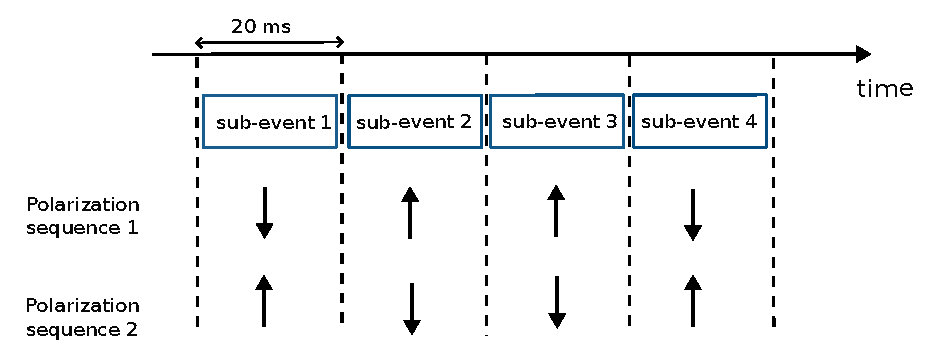
\includegraphics[width = 0.75\textwidth]{ExperimentalSetup/EventStructure.pdf}
\caption{General structure of the event. The gate-length of each event is synchronized with the power grid frequency, to reduce possible effects of $\SI{50}{\hertz}$ noise.}
\label{fig:EventStructure}
\end{figure}

The particular choice of $\SI{20}{\milli \second}$ for the sub-event is made to avoid undesirable effects generated by the power grid frequency ($\SI{50}{\hertz}$). The gate-length of each sub-events is synchronized with the period of the power grid frequency: this ensures that an entire oscillation of the current of the power grid takes place within the same sub-event. This cancels out the $\SI{50}{\hertz}$ noise and avoid to produce effects between nearby sub-events.
For each event we have a single measurement of $A_{n}$, defined as the asymmetry between the $\uparrow$ and $\downarrow$ sub-events. It is important to avoid the creation of fake asymmetries by correlated noise or other external sources. For this reason polarization states are concatenate following the two patterns $\uparrow, \downarrow, \downarrow, \uparrow$. In addiction at the beginning of an event one of the two polarization pattern is selected using a De Bruijn sequence. A De Bruijn sequence of order n is defined as a cyclic sequence where every sub-sequence of length n appear only once. We have two different polarization pattern, the ones shown in the figure, that can be represented as $1$ and $0$. For this experiment, the De Bruijn sequence is of order $n = 6$ bits; this correspond to all the possible sequences of $1$ and $0$ with a length equal to $6$, which are $64$ different sub-sequence.
It is possible to demonstrate that the number of exactly $N_{De Bruijn}$ sequences is: 
\begin{align*}
N_{bruijn} = \frac{(k!)^{k^{n-1}}}{k^{n}}
\end{align*}
If we substitute in the formula above $k=2$ and $n = 6$, we have a total of $\simeq 67 \cdot 10^{6}$ different sequences. The seed of the De Bruijn sequence is generated with a pseudo random number generator, and the sequence is used to select between $\uparrow,\downarrow,\downarrow, \uparrow$  and $\downarrow,\uparrow,\uparrow,\downarrow$. At this point it could be objected why so much care is taken in choosing randomly the two sequences. At a first glance is certainly easier to select one of the two polarization pattern and reproduce it for every sub-event. However, this does not protect from systematic effects that arise from electronic or beam noise with frequencies similar to the frequency of the polarization pattern.  
An electronic noise, with a frequency roughly $\SI{10}{\hertz}$ could in principle increase the rates for one polarizations state and decrease the other. The adopted solution to reduce possible effect is to randomize the pattern selection. In the end, there is another reason why a De Bruijn sequence is useful. During each polarization flip, we observe a short, transient reduction of the beam current. This reduction in the beam intensity has more influence on patterns where there are more inversion of the polarization respect to the other. With a De Bruijn sequence we ensure that we have a identical number of pairs of patterns, meaning that:

\begin{itemize}
\item $25\%$ : $\uparrow,\downarrow,\downarrow, \uparrow$ ; $\uparrow,\downarrow,\downarrow, \uparrow$
\item $25\%$ : $\downarrow,\uparrow, \uparrow,\downarrow$ ; $\downarrow,\uparrow, \uparrow,\downarrow$
\item $25\%$ : $\downarrow,\uparrow, \uparrow,\downarrow$ ; $\uparrow,\downarrow,\downarrow, \uparrow$
\item $25\%$ : $\uparrow,\downarrow,\downarrow, \uparrow$ ; $\downarrow,\uparrow, \uparrow,\downarrow$
\end{itemize}

In the top rows we have 4 inversion, while in the two lower rows we have 5 inversion. \smallskip
Later we will describes the other details of the experiment; in the next sections we will present briefly MAMI accelerator, where the experiment is performed. 

\section{Mami}

MAMI is the electron accelerator located in Mainz, which provides a continuous wave \footnote{The electron beam is made by bunches of electrons, in sequence. In MAMI the separation between subsequent bunches is so small that it is not possible, with the available instrumentation, to distinguish it from a continuous flow of particles.}, high intensity, polarized beam for nuclear physics fixed-target experiments. The concept of the Mainz microtron accelerator was born in the early 1970s, when the researchers of the nuclear physics institute were investigating the possibility of generalizing the concept of the racetrack microtron (RTM), that consists in a linear accelerator (linac) and two deflection magnets ($180^{\circ}$ magnet, see figure \ref{fig:RaceTrackSketch}). The particle recirculate, due to the deflection magnets, several time in the linac, and each time they gain energy.  The goal of the collaboration which developed MAMI was to produce a continuous beam, with energies above $\SI{1}{\giga \electronvolt}$ and beam intensities up to $\SI{100}{\micro \ampere}$.

\begin{figure}[hbtp]

\centering
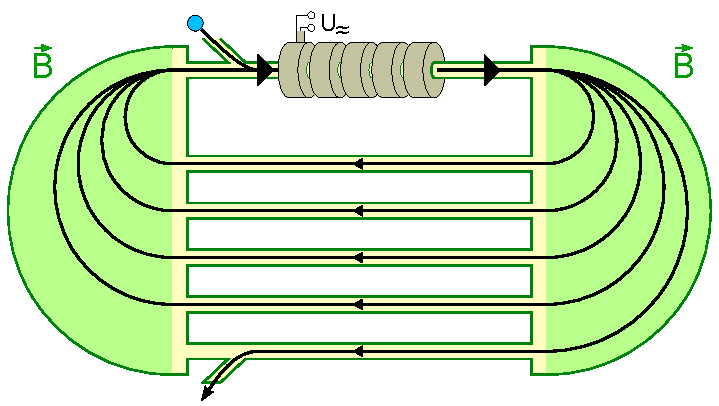
\includegraphics[width = 0.75\textwidth]{ExperimentalSetup/RacetrackMicrotronSketch.pdf}
\caption{Racetrack Microtron. The particles are sent to the linac, and the two deflection magnets make the particles recirculate, until the momenta exceed the capability of the magnetic field.}
\label{fig:RaceTrackSketch}
\end{figure}

A racetrack microtron, is characterized by the energy gain per-cycle $\delta E$ given by the high-frequency electromagnetic field (HF). The energy gain for a single acceleration cavity of the linac is: 

\begin{align*}
\delta E \, = \, e U_{Linac} \cdot cos(\phi)
\end{align*} 

$U_{Linac}$ is the maximum voltage of the linac, and $\phi$ is the phase of the beam relative to the maximum of HF. Because the particle are accelerated by the linac, the beam consist in individual packets (bunches) whose rate correspond to the frequency of HF. In order for the electrons to be accelerated for each recirculation step, they must arrive at the beginning of the linac with the correct phase $\phi$. Therefore the flight-time per cycle must be an integer or a multiple of the HF period. The time of flight is made of two terms: the first is the time that an electron needs to travel in the magnetic field of two $180^{\circ}$ bending magnets, that is the cyclotron period, while the second term is given by the straight sections. 

\begin{equation} \label{eq:TimeofFlight}
T = \dfrac{2 \pi \gamma m_{e} }{qB} + \dfrac{L}{v}
\end{equation}

where $B$ is the magnetic field, $q$ and $m_{e}$ are the charge and mass of the electron, and $L$ is the length of the straight section of the accelerator. The frequency is the given by the formula:

\begin{equation} \label{eq:frequency}
f = \dfrac{qB}{2 \pi \gamma m_{e} + \frac{LqB}{v}} 
\end{equation}

From this overview two conclusion can be drawn:

\begin{itemize}
\item To accelerate slow electrons, with $\gamma = (1,10)$, a magnetic field of $\SI{0.1}{\tesla}$ is used, in order to work with frequencies of ($\SI{2}{\giga \hertz}$,$\SI{4}{\giga \hertz}$), that are easy to control. However with higher energies, and with a small magnetic field, the bending radii is higher and uneconomical.
\item For high energy electrons $\gamma > 10$, to reduce the size of the deflection magnets, it is useful to increase the magnetic field up to $\SI{1}{\tesla}$ of more, with the same band of frequencies $\simeq \SI{}{\giga \hertz}$.
\end{itemize}

These conclusions justify the structure of MAMI: a cascade of microtrons to reach each time higher energies with the same acceleration frequency at each stage.
MAMI is composed by a sequence of 4 different microtrons, reaching $\SI{1.6}{\giga \electronvolt}$. 

\begin{figure}[hbtp]
\centering
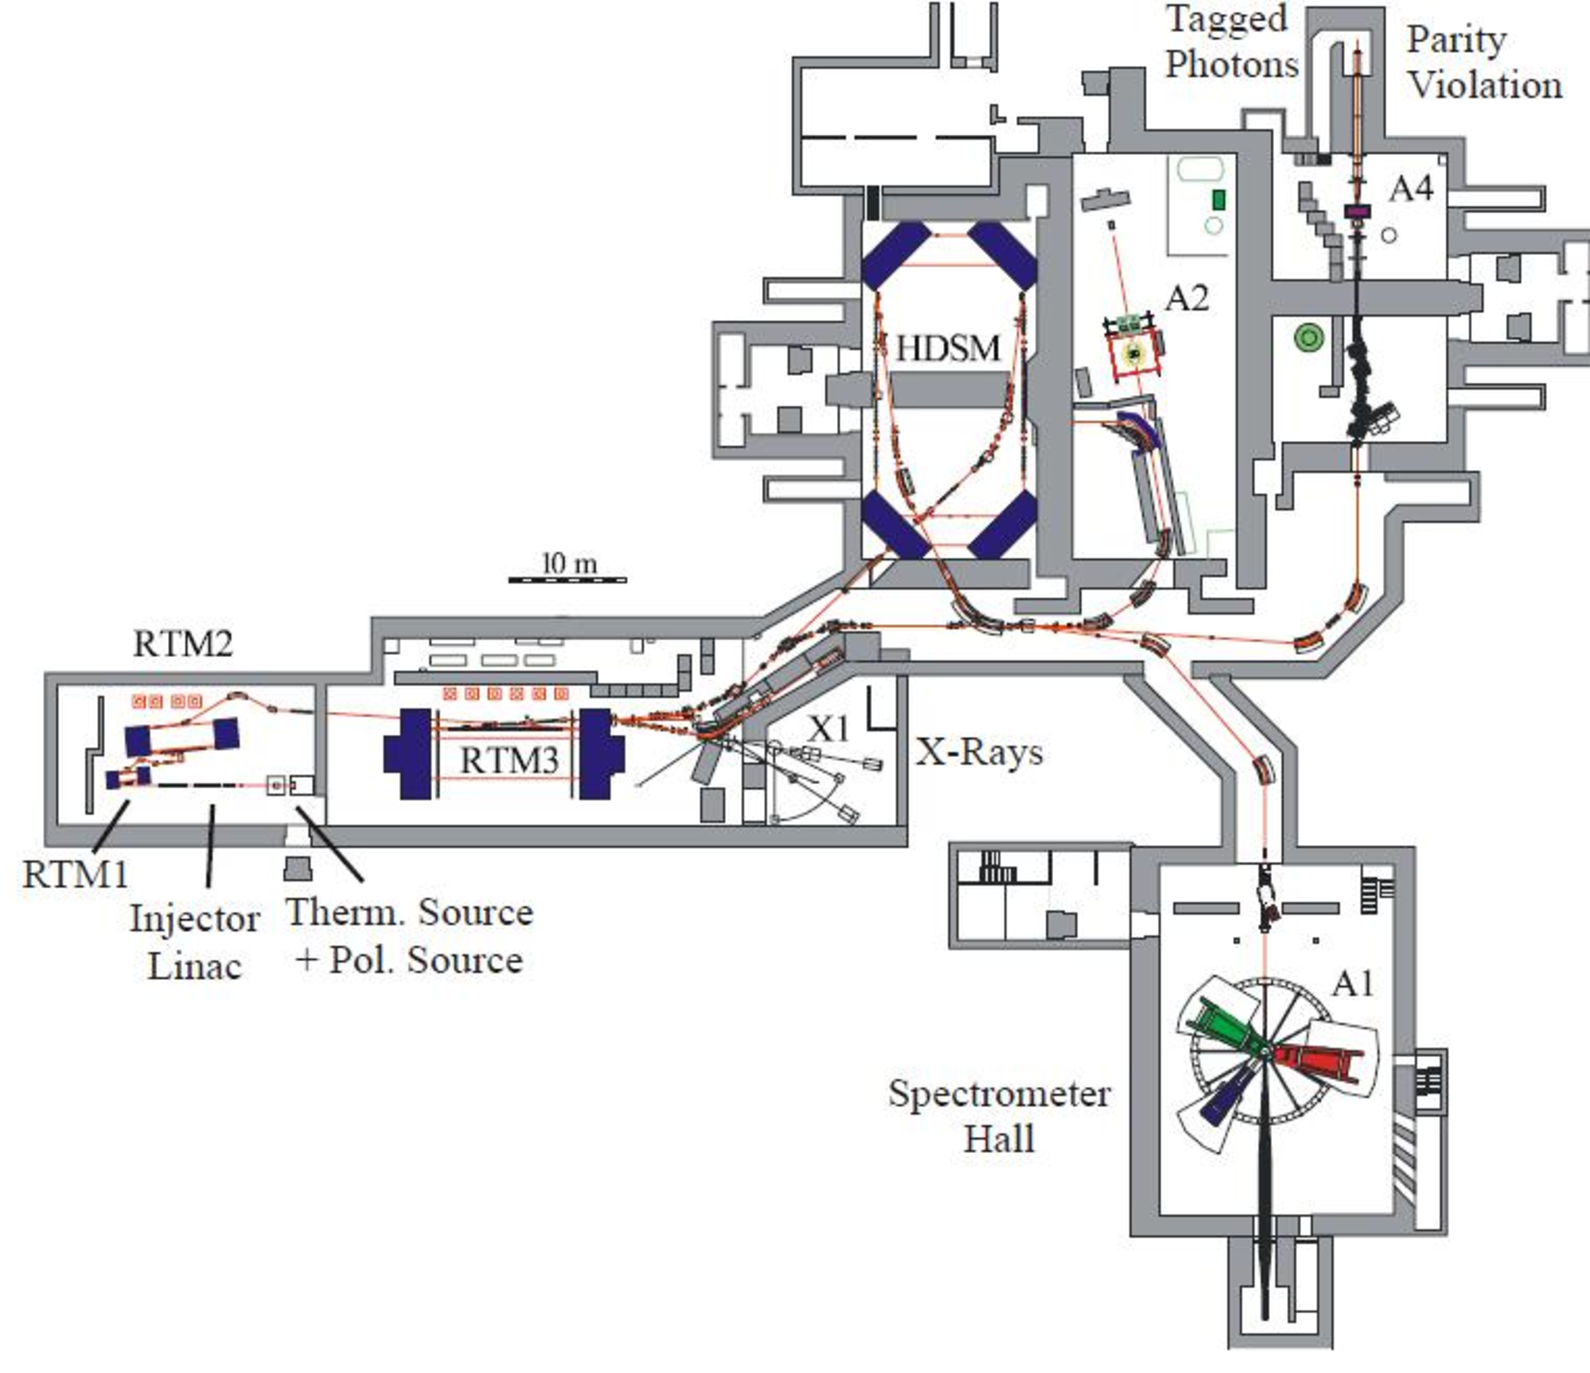
\includegraphics[width = 0.6\textwidth]{ExperimentalSetup/Accelerator.pdf}
\caption{Scheme of the accelerator, with the different experimental halls. A third hall previously used for the A4 experiment, measuring the strange quark content of the proton, is now being used for the novel MESA accelerator and its experiments.}
\label{fig:Accelerator}
\end{figure}

The first stage, shown in figure \ref{fig:Accelerator}, is composed by two small microtrons. The first microtron RTM1 accelerate the particles to $\SI{14}{\mega \electronvolt}$ in 18 revolutions. The electrons are then sent to the second microtron that can accelerate up to $\SI{180}{\mega \electronvolt}$. After passing the first stage, the beam is sent to the RTM3 (race track microtron 3), a large microtron with an end point energy of $\SI{855}{\mega \electronvolt}$. These 3 microtrons forms MAMI-B, which started operation in 1990-91. A fourth stage, MAMI-C, was built and started operation in 2007. This fourth stage is made by 4 bending magnets, with a bending angle of $90^{\circ}$, and it is designed to achieve energies of $\SI{1.6}{\giga \electronvolt}$. The design is different from the other race-track microtrons, and will not be explained, as it is not necessary for the experiment to reach such high energies.

\begin{figure}[hbtp]
\centering
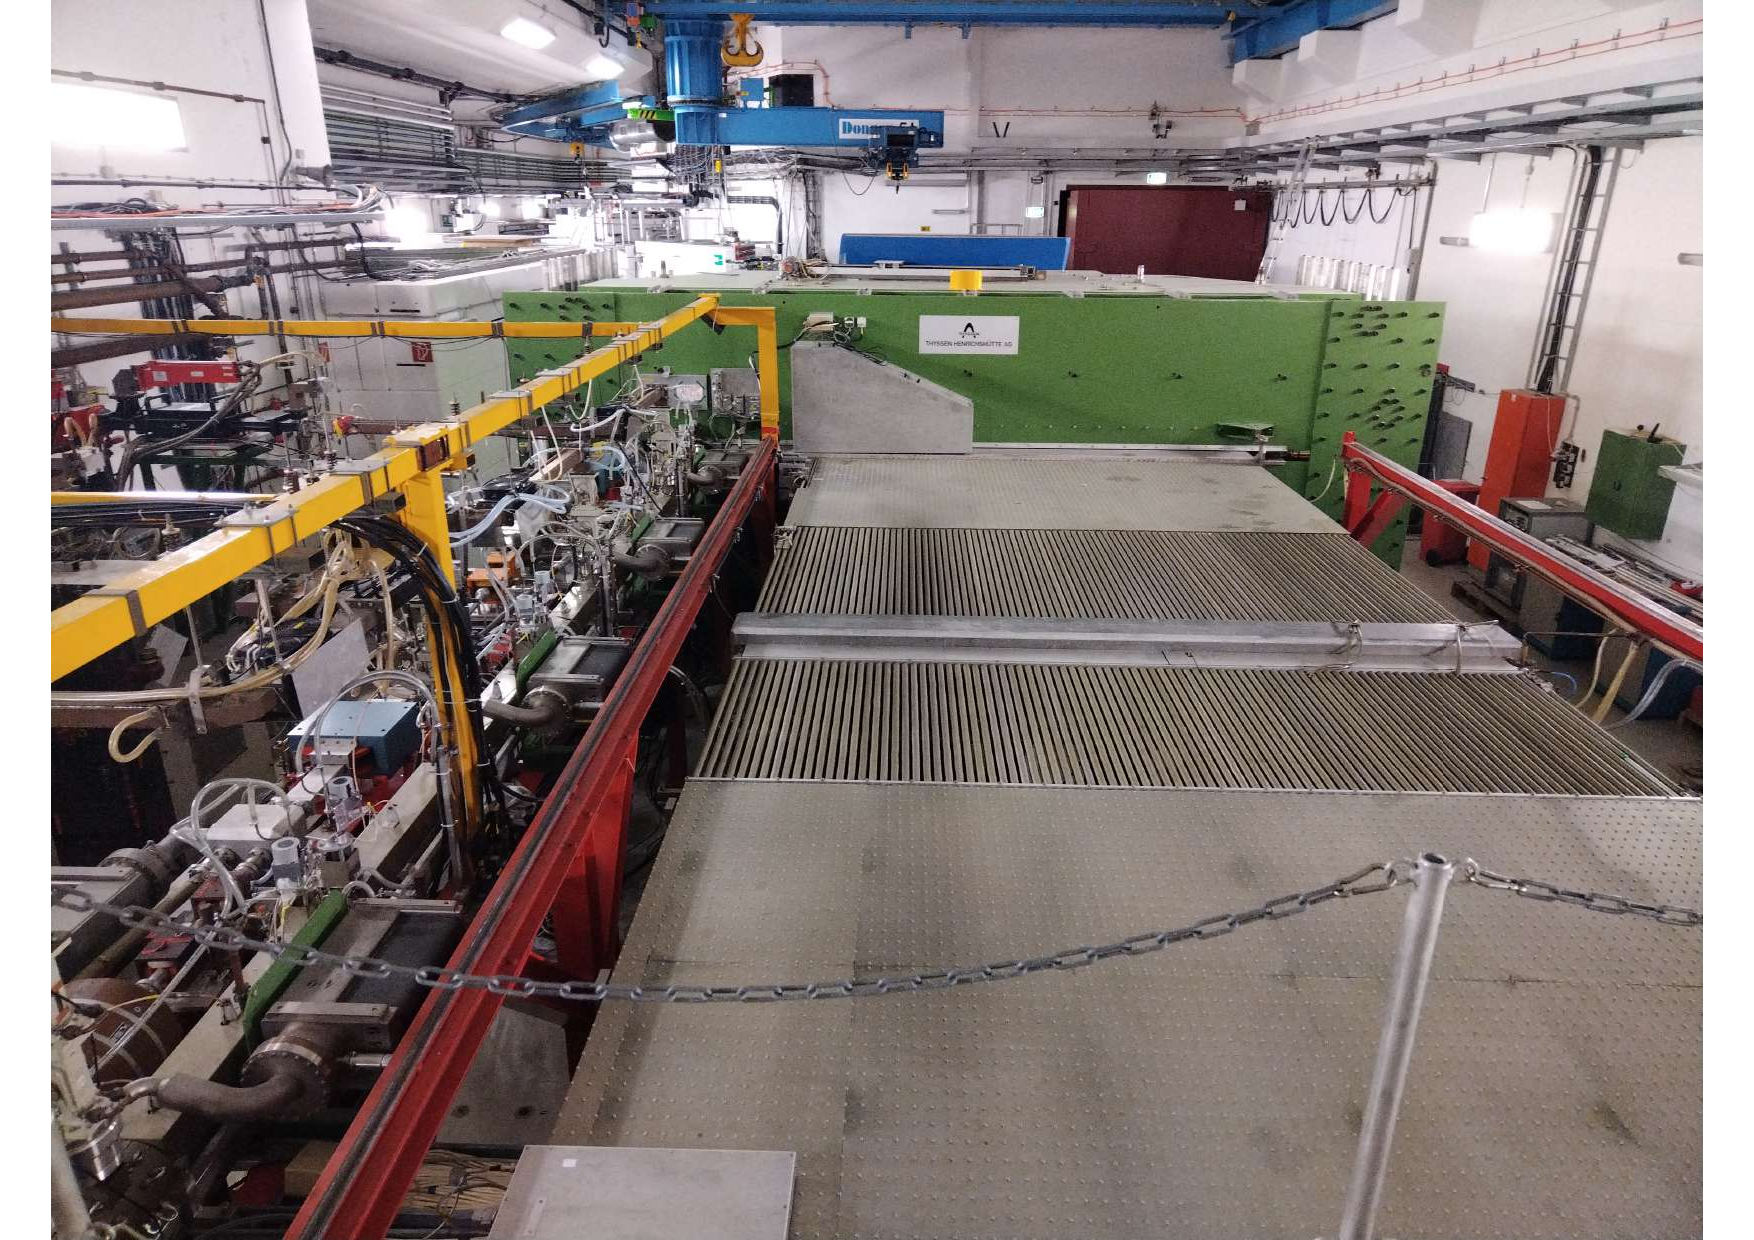
\includegraphics[width=0.75\textwidth]{ExperimentalSetup/Racetrack.pdf}
\caption{Picture of the Racetrack RTM3 in MAMI-B. The Green square at the bottom is one of the deflector magnets, the other one is below the point where the photo was taken. The linac stage is on the left. The tubes at the center of the figure are the paths that the particle cross during the recirculation. The further away from the linac the greater the energy.}
\end{figure}

The operation principles of a microtron are simple to be described. First we consider the gyro-radius for relativist electrons of energy $E$, that is:

\begin{equation}
\qquad r = \dfrac{E \beta}{qcB}
\end{equation}

To have a coherent conditions, we must have that the flight-time $\tau = \frac{\lambda}{c}$ of the first recirculation must be an integer multiple of the HF wavelength $\lambda_{HF} = \frac{c}{f_{HF}}$, see equation \ref{eq:frequency}. This means that:

\begin{align*}
\lambda = \tau c =\dfrac{ 2 \pi c R }{\beta c} + \frac{Lc}{v} = \dfrac{2 \pi E}{q B} + L = m \lambda_{HF}
\end{align*}

For the other recirculation, we must have that the flight-time at energies $E_{n} = E_{n-1} + \delta E$ must be increased by an integer multiple of HF, too. This lead to the second equation:

\begin{align*}
\dfrac{2 \pi \delta E}{q B} = n \lambda_{HF}
\end{align*}

The minimum gain per cycle is then determined only by the strength of the magnetic field and wavelength $\lambda_{HF}$. These two equations together controls the dynamic of the race-track microtrons.

\subsection{Polarized Beam}

For the beam-normal single spin asymmetry a vertically polarized beam is necessary. At the MAMI electron accelerator it is possible to produce a vertically polarized beam with energy in the range $\SI{180}{\mega \electronvolt} - \SI{855}{\mega \electronvolt}$ \cite{Schlimme:2016rrp}. In this section the procedure to orient the spin vertically is presented, following an explanation of how the degree of polarization is measured. \smallskip

The electron source used at MAMI is made by a strained GaAs/GaAsP super-lattice photo-cathode illuminated by circularly polarized light. To alternate the sign of the light polarization, a fast Pockels cell (\cite{Goldstein}) is installed in the optical system of the electron source. The Pockels cell is a wave plate controlled by the electric field, that changes the helicity of the photons impinging on the electrons. A Pockels cell exploits the Pockels effect, that affects crystal with particular characteristics (lack of inversion symmetry). For this type of materials the refractive index is linearly dependent on the applied electric field. By controlling the refractive index with the electric field, the polarization state of the incident light beam is altered.
The extracted electron carries the same helicity of the incoming photon because of angular momentum conservation:
\begin{center}
\begin{equation}
\feynmandiagram [scale = 0.8, transform shape][baseline = (g)]{
	a [particle = \(e^{-}\)] -- [fermion] b  -- [fermion] c [particle = \(e^{-}\)],
	b -- [boson] d [particle = \(\gamma\)],};
\hspace{2cm}
(Jz)_{\gamma} = \pm 1 \qquad (Jz)_{e^{-}} = \mp \frac{1}{2} \rightarrow \pm \frac{1}{2}
\end{equation}
\end{center}

With the fast change of the Pockels cell it is possible to alternate the sign of the polarization. By the insertion of a $\lambda/2$ plate between the laser system and the photo-cathode the global polarization orientation of the electron beam can be reversed. This is particularly useful because this directly changes the sign of the asymmetry measured by the detectors, and allows to identify systematic errors. This is usually done for longer beam time, where two sets of data are taken, reversing the orientation of the $\lambda/2$  wave plate. By comparing the results for the two sets of data, the influence of the optical system on the asymmetry measurement is estimated and can be corrected for the final result of the asymmetry. During the beam time of interest for this thesis, the $\lambda/2$ wave plate orientation was fixed. The beam polarization achieved with this source is roughly $P = 80 \% $, so the measured asymmetry are:

\begin{align*}
A_{measured} = P \cdot A_{n}
\end{align*}

The polarizations of the electrons just extracted from the source is longitudinal. A magnetic field is needed to rotate $\vec{P}$ from longitudinal to transverse orientation. For this purpose two devices are used: the \textbf{Wien filter} and a double solenoid located in the injection beam line, close to the the optical source, as show in figure \ref{fig:Iniezione}:

\begin{figure}[hbtp]
\centering
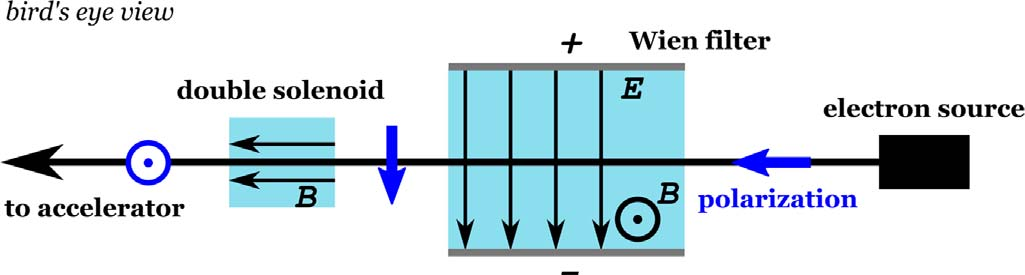
\includegraphics[width = \textwidth]{ExperimentalSetup/injection.png}
\caption{Beam line projection. This figure is taken from the paper \cite{Schlimme:2016rrp}}
\label{fig:Iniezione}
\end{figure}

Looking at the picture, the longitudinal direction corresponds to the $Z$ axis. The $X$ axis is parallel to the second blue arrow, just after the Wien filter, and the $Y$ axis is orthogonal to the page. 
The spin is rotated primarily in the $X$ direction, with a $90^{\circ}$ rotation, then the subsequent double solenoid align the spin to the vertical direction, with another $90^{\circ}$ rotation. 
Once the beam passes the double solenoid, the electrons go through the linac, the microtron and in the end to the experimental hall, where the target of the experiments is installed. During the acceleration stage, the spin follows the precession motion due to the various magnetic fields of the accelerator, as determined by the BMT equation. However in our experimental setup, the magnetic field of the various bending magnets that constitute the microtron-cascade are always parallel to the polarization in vertical direction, so that the cross product $\vec{B} \times \vec{P} = 0$, and the polarization remain constant. Only the residual horizontal component precedes during the motion. For conventional experiment that involve longitudinal polarization, after the first spin rotation due to Wien filter and the bending magnets, there is a further rotation to be considered, due to the motion of the particle during the acceleration and recirculation in the microtron. Because of this, the rotation made by the Wien is set in such a way that after the second rotation due to the motion in the accelerator, the polarization has the correct alignment in the experimental hall. The rotation angles of the polarization vector through the accelerator are known from simulations and are also directly measured for relevant energies, for a beam of $\SI{570}{\mega \electronvolt}$ the rotation angle is $\ang{55}$ with an accuracy of $\pm \ang{2}$. In our case, this further rotation has only a small effect to the residual horizontal component. This horizontal component was accurately minimized by MAMI operators at the beginning of the beam time, and its effects the measurement are negligible. MAMI was not developed for experiments with transverse polarization. So it's not possible to measure directly the transverse component. However the vertical polarization is deduced from the determination of the total beam polarization and the residual horizontal components. For this purpose a Moller, Comport and Mott polarimeters are used.

\subsection{Vertical Polarization Measurement}
Three polarimeters are installed in MAMI: Mott, M\o ller and Compton polarimeters. Compton and Mott polarimeter are located behind the injector linear accelerator (see figure \ref{fig:Accelerator}), close to the beam source, where the electrons, with an energy of $\SI{3.5}{\mega \electronvolt}$, have already passed the Wien filter and the double solenoid. The M\o ller polarimeter, instead, is installed in the spectrometer hall, where the beam is delivered. The M\o ller polarimeter is sensitive only to the longitudinal component of the polarization, while the Mott and Compton polarimeter are sensitive to the $Z$ and $X$ component. 
When the beam is polarized longitudinally, the total polarization can be measured by a M\o ller polarimeter, in the spectrometers hall. The procedure for the alignment is the following: at the beginning of the beam time the Mott polarimeter is used for different settings of the solenoid field, with the Wien filter angle equal (nominal) to $\ang{90}$. The aim is to minimize the horizontal polarization component ($P_{x}$) after the rotation performed by the double solenoid, changing the solenoid magnetic field. Then a second minimization follows, using the M\o ller polarimeter and changing Wien filter  rotation angles. In this way we minimize also the longitudinal component ($P_{z}$). With the new Wien filter settings, another measurement is performed with the Mott polarimeter. With this procedure, the $P_{x}$ and $P_{z}$ components are completely minimized, with the result that the beam polarization is parallel to the $Y$ axis.
At this point, the polarization is correctly aligned, and the experiments can start. The last polarimeter, the Compton, is used to measure the variation of the degree of polarization during time. 

In the last measurement of $A_{n}$ at MAMI \cite{Esser:2018vdp} the Moller and Mott polarimeters were available. In this way, it is also possible to estimate the systematic uncertainty for the degree of polarization, which is the relevant contribution to the total systematic uncertainty of the final measurements of $A_{n}$. The systematic effects obtained during the previous experiment were about $1 \, ppm$. For the experiment described in this thesis, we performed the minimization described before only with the Mott polarimeter, obtaining a measure of the transverse polarization $P = 0.79\%$. This means that we could not estimate the systematic uncertainty of the polarization.

\subsection{Mott Polarimeter}

In this section we describe the theory of the Mott polarimeter. The Mott polarimeter exploits the asymmetry in the cross section due to the spin dependence. From the asymmetry we can to measure the polarization of the beam. 
Let's suppose that we have an electron beam that is sent towards a nucleus of charge $Ze$. We know from theory \cite{MottElectron} that the spin of the incident electron interacts with the electromagnetic field produced by the nucleus.
The magnetic field seen by a particle with speed $\vec{v}$ near a nucleus is:

\begin{align*}
\vec{B}_{nucleus} = \frac{-\vec{v} \times \vec{E}_{nucleus}}{c}  = \frac{Ze}{mc r^{3}} \vec{L} 
\end{align*}

This magnetic field is coupled with the magnetic momenta of the electron $\mu_{e}$.

\begin{equation}
V = - \vec{\mu} \cdot \vec{B}_{nucleus} = \frac{Ze}{mcr^{3}} \vec{L} \cdot \vec{S}_{e^{-}}
\end{equation}

The second equation represents the spin-orbit interaction potential. This term yields the polarization dependence of the cross section. Let's consider an incident particle that scatters from a nucleus at an angle $\theta$, as shown in the figure:

\begin{figure}[hbtp]
\centering
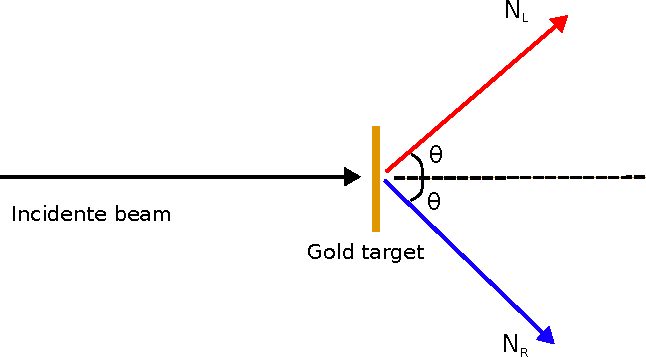
\includegraphics[width = 0.45\textwidth]{ExperimentalSetup/MottScattering.pdf}
\caption{Scheme of the Mott scattering, the polarization is orthogonal to the plane,  $ \vec{n} = \frac{\vec{k} \times \vec{k'}}{|\vec{k} \times \vec{k'}|}$}
\label{fig:MottScatt}
\end{figure}

The cross section can be modeled highlighting the dependencies on the polarization $\vec{P}$:

\begin{equation} \label{eq:MottCross}
\dfrac{\partial\sigma(\theta)}{\partial \Omega} = I(\theta) [1 + S(\theta) \vec{P} \cdot \vec{n} ]
\end{equation}

In the equation above, the cross section is divided in two terms: $I{\theta}$ represents term that does not depend on the polarization, the second contains the dependence on the polarization, where $S(\theta)$ is the Sherman function, or the asymmetry function \cite{10.1063/1.1143371}. The unit vector $\vec{n}$ is normal to the scattering plane, and it is defined as:

\begin{align*}
\vec{n} = \dfrac{k \times k'}{|k \times k'|}
\end{align*}

Where $k$ and $k'$ are the wave vectors associated with the incident and scattered electrons. The direction of $\vec{n}$ is parallel to the angular momentum $L$, and depends on whether scattering to the left or to the right is being considered.
Let's suppose our initial beam has a polarization $P$, that can also be expressed as:

\begin{align*}
P = \frac{N_{\uparrow} - N_{\downarrow}}{N_{\uparrow} + N_{\downarrow}}
\end{align*}

Where $N_{\uparrow}$ and $N_{\downarrow}$ are the number of electrons with spin up and spin down. The Mott polarimeter measure the number $N$ of scattered electrons at a fixed angle $\theta$, in the two directions right and left (figure \ref{fig:MottScatt}). Using the equation \ref{eq:MottCross}, the scattered electrons to the left side $N_{L}$ and to the right side $N_{R}$ are equal to: 

\begin{align*}
N_{L} &= N_{\downarrow}[1 + S(\theta)] + N_{\uparrow}[1 - S(\theta)] \\
N_{R} &= N_{\uparrow}[1 + S(\theta)] + N_{\downarrow}[1 - S(\theta)]
\end{align*}

The asymmetry $A(\theta)$ of the scattered electron between left ($N_{L}$) and right ($N_{R}$) is given by:

\begin{align*}
A(\theta) = \frac{N_{L} - N_{R}}{N_{L} + N_{R}} &= \dfrac{N_{\downarrow}(1 + S(\theta)) + N_{\uparrow}(1 - S(\theta)) - N_{\uparrow}(1 + S(\theta)) - N_{\downarrow}(1 - S(\theta))}{N_{L} + N_{R}} = \\ 
&= \dfrac{(N_{\uparrow} - N_{\downarrow})}{(N_{\uparrow} + N_{\downarrow})}S(\theta) =  P \cdot S(\theta)
\end{align*}

The last step of the equation gives the beam polarization in terms of $A(\theta)$, the asymmetry measured by the Mott polarimeter, and the function $S(\theta)$, the Sherman function. The Mott polarimeter in MAMI, installed after the double solenoid, measures the scattering asymmetry $A(\theta)$ for electrons of $\SI{3.5}{\mega \electronvolt}$ with a thin gold target.  

\newpage
\section{Experimental Hall Setup}

Until now we have described how MAMI produce to accelerate the electrons, however we have not presented the structure where the beam is delivered and various experiments are carried out.
MAMI experimental halls are named with the capital letter A followed with a number. In A2, for example, photo-nuclear reactions are studied to investigate the fundamental physics at the scale of nuclear dimensions. The experimental hall where the experiment described in this thesis is conducted is the A1 hall. We will describe briefly the main operating detectors that are installed and the details that are interesting for the transverse asymmetry measurement.
In A1 hall the beam is delivered with energy in a range starting from $\SI{180}{\mega \electronvolt}$ up to $\SI{1.6}{\giga \electronvolt}$. Energy greater than $\SI{855}{\mega \electronvolt}$ are reached with the last acceleration stage HDSM, shown in figure \ref{fig:Accelerator}. Because the electron energy of our experiment is $\SI{570}{\mega \electronvolt}$, the beam passes only through the first acceleration steps, and is extracted from the RTM3 and directly sent to the A1 experimental hall, without going through the HSDM stage. 

\begin{figure}[!h]
\centering
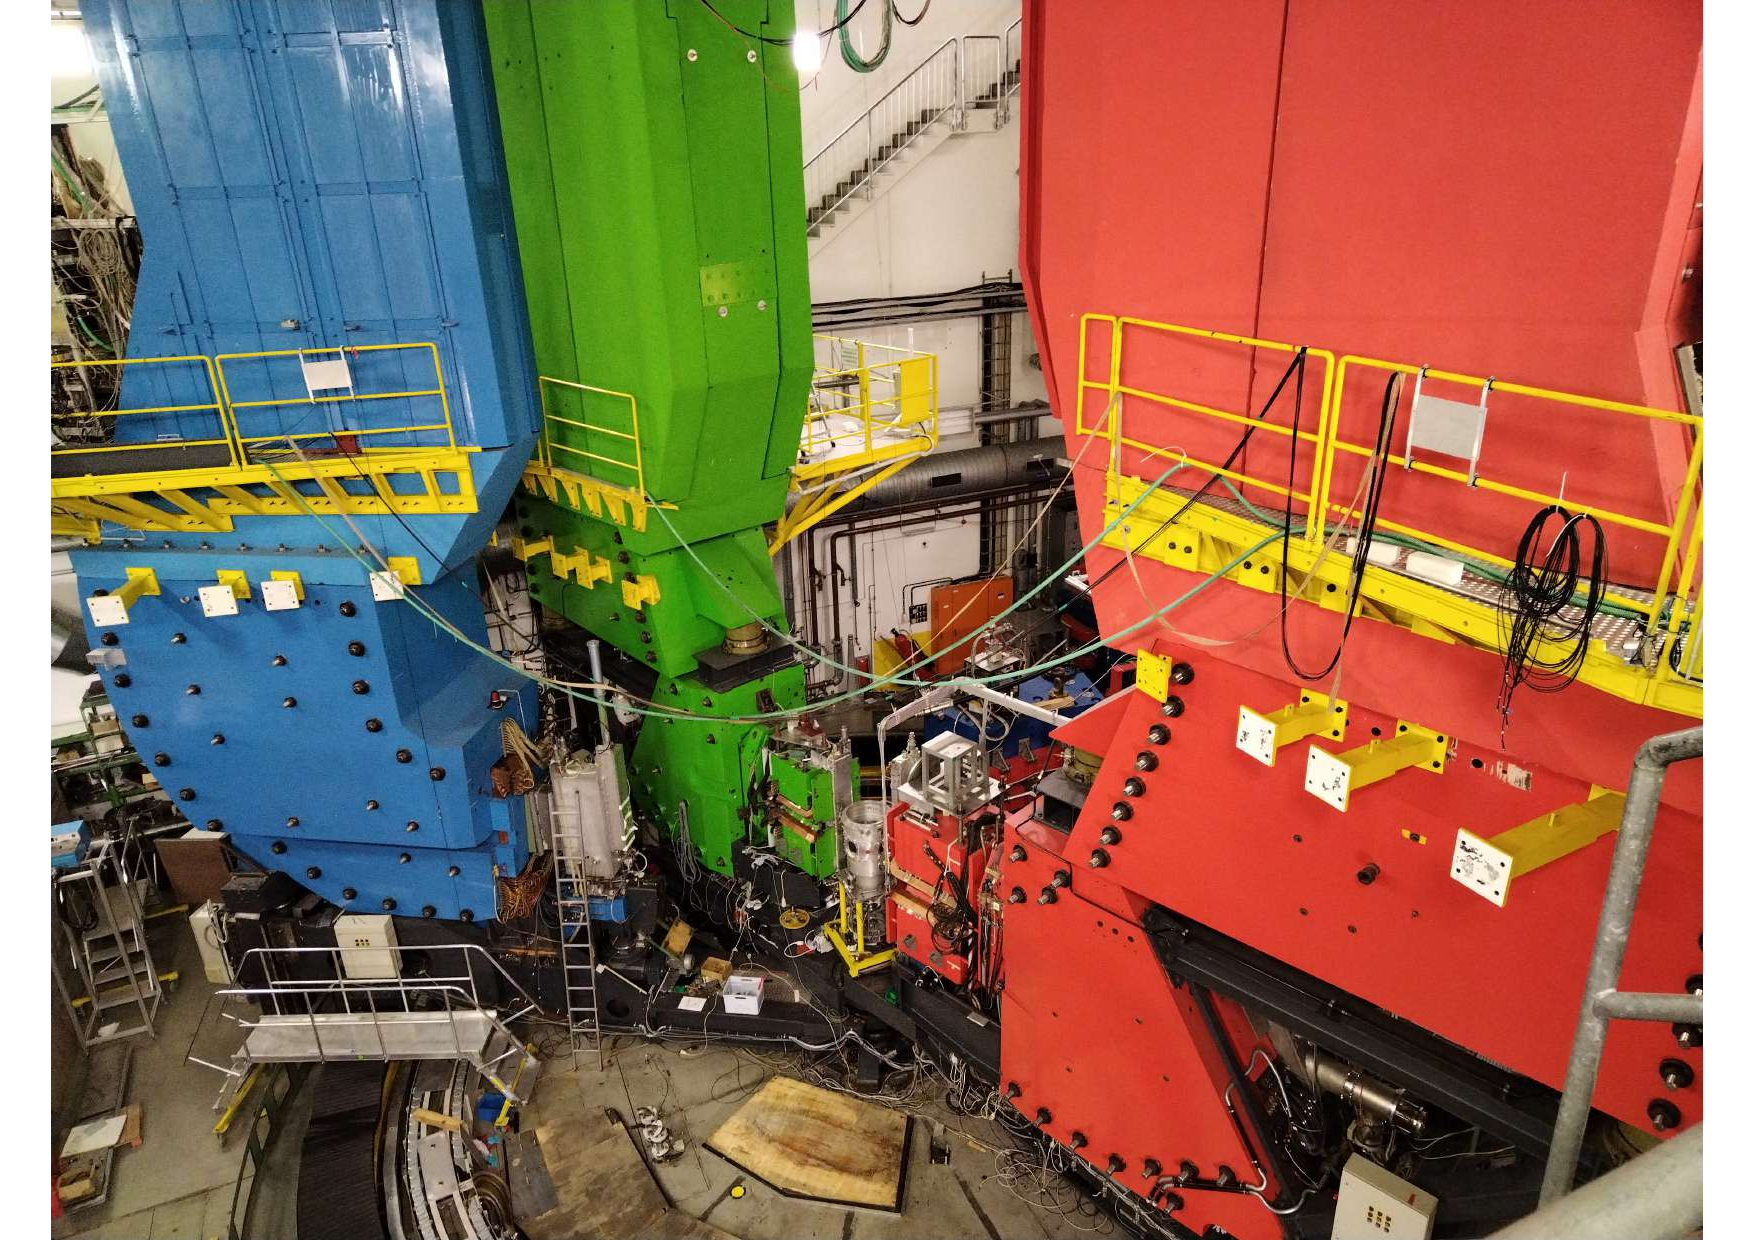
\includegraphics[width = 0.9\textwidth]{figures/twoSpektrometer.pdf}
\caption{Picture of the A1 spectrometers hall, the spectrometers red and blue are used during this experiment. At the center of the picture is possible to observe the scattering chamber.}
\label{fig:TwoSpektr}
\end{figure}

Inside A1 hall three large magnetic spectrometers are placed on a circular rail-track around the target chamber (figure \ref{fig:TwoSpektr}). They where designed and built in $1993$ to perform high precision measurement of electron scattering in coincidence with other hadron detection, with an high resolution in the determination of the particle momenta $\frac{\delta p}{p} < 10^{-4}$. The spectrometers develop vertically with a height of $\SI{15}{\meter}$, for this reason the scattered electrons and the other particles are deflected with respect to the scattering plane with the use of magnetic fields. The figure \ref{fig:TwoDetectors} shows the path of the particles scattered from the target. The spectrometers used for the transverse asymmetry measurement are the red and blue ones. There are multiple reasons why the particle are deflected on the vertical direction, we summarized them in two points: 

\begin{itemize}
\item reason of space, due to the fact that a horizontal setup would not fit with the dimension of the building in addiction to the fact that this would not allow to rotate the spectrometers by a variety of angles that the vertical orientation does
\item reduce background and noise, in fact the high beam intensity that is possible to reach at MAMI is a source of noise and background event which can be cut off detecting the particle far from the interaction point.
\end{itemize}    

\begin{SCfigure}[30][!ht]
\centering
\caption{Image of the spectrometers of A1 hall. The spectrometers can be rotated using a system of rail-tracks that are visible at the bottom of the image. The electrons are scattered and then deflected in the vertical direction by the magnetic field (green lines). This picture is taken from behind the target. The target is roughly at the center of the image where the two green lines join. The electron are coming from the opposite direction, with respect to the spectrometers.}\label{fig:TwoDetectors}
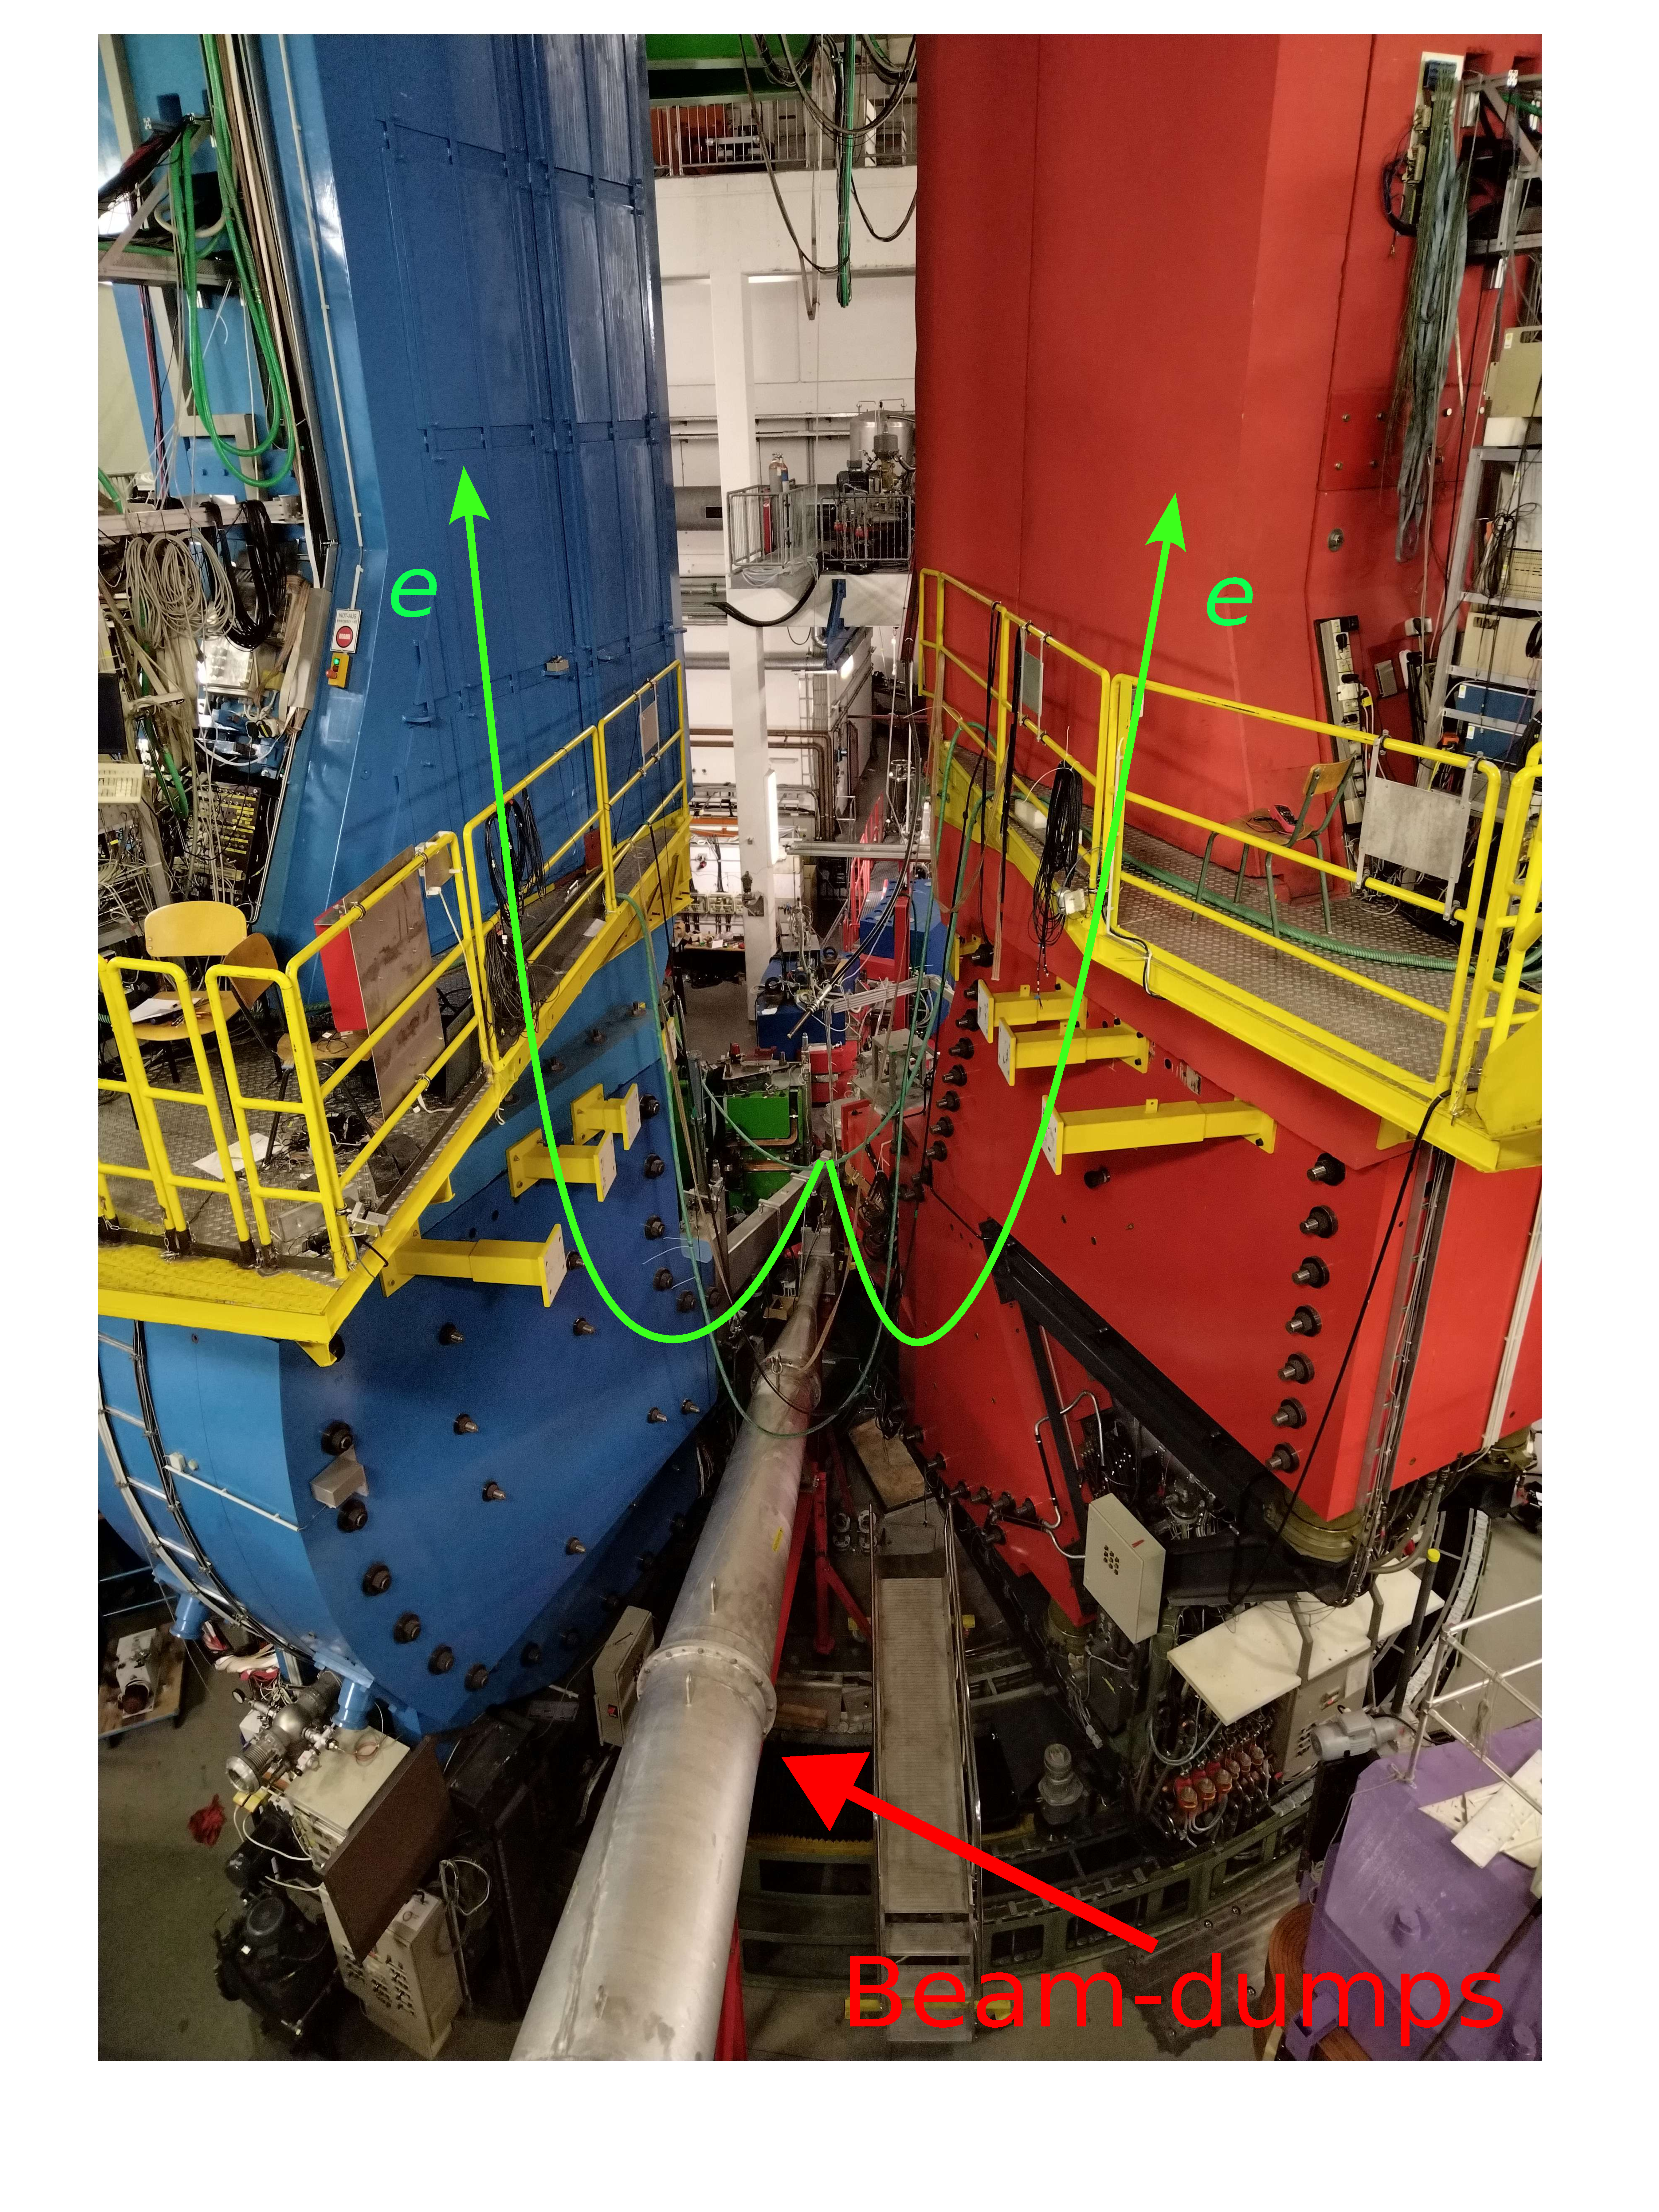
\includegraphics[width = 0.5\textwidth]{ExperimentalSetup/A1_Dietro.pdf}
\end{SCfigure}
  
Once a particle is scattered in the acceptance region of the spectrometers, it is deflected by the magnetic field and passes through the drift chamber, which occupies the first third in height of the spectrometers. 
When the particle is at the height of the platform in the figure \ref{fig:TwoDetectors}, it impinges on a layer of plastic scintillator, and after that a Cherenkov detector  measures the particle speed $v$. In figure \ref{fig:internal} the spectrometer A internal, taken during the installation of detector A, is shown. The determination of both the particle speed $v$ and momenta (drift chamber) allows particle identification.
\begin{SCfigure}[30][!h]
\centering
\caption{Internal of the spectrometer. This image was taken during the installation of the detector A inside the red spectrometer, that is accessible from the platforms visible in the picture \ref{fig:TwoDetectors}}
\includegraphics[width=0.30\textwidth]{ExperimentalSetup/Detectors/position.pdf}
\label{fig:internal}
\end{SCfigure} 

Despite the possibilities offered by the already existing setup, for the beam time of interest none of these components was used directly in the estimation of $A_{n}$. The reason is due to the high intensity of the beam that is used in the experiment, which is far from the optimal operating conditions of the components, that are suited for rates lower than the ones expected for beam normal single spin measurements. The spectrometers are used indirectly, for the alignment of scattered electrons to our detection system.


\section{Detector Description} \label{detectors}
In this section we will describe the electronics and the detectors used to measure the transverse spin asymmetry.
For this experiment we are going to measure the transverse asymmetry at one fixed angle, corresponding to a transferred momentum of $Q = \SI{0.2}{\giga \electronvolt}$. The electrons detection is 
made via two thin blocks of fused-silica that are coupled to PMTs. When a scattered electron hits the fused-silica (refractive index $n = 1.45$) Cherenkov light is emitted. The emitted Cherenkov light can extract one electron in the photocathode, which will be amplified by the PMT dynode structure. This sequence of event triggers the PMT and produce an output signal.

In the experiment two detectors are installed and read-out independently. The detector A is placed at an angle of $+\theta$, while detector B is placed at $-\theta$. We expect to measure the same absolute value of the transverse asymmetry, with an opposite sign due to the different orientation. 
The two detector are made by 3 PMTs and 8 PMTs coupled with two blocks of fused-silica, as shown in \ref{fig:NostriDetector}:

\begin{figure}[hbtp]
\centering
\subfloat[][\emph{Detector B scheme.}]{
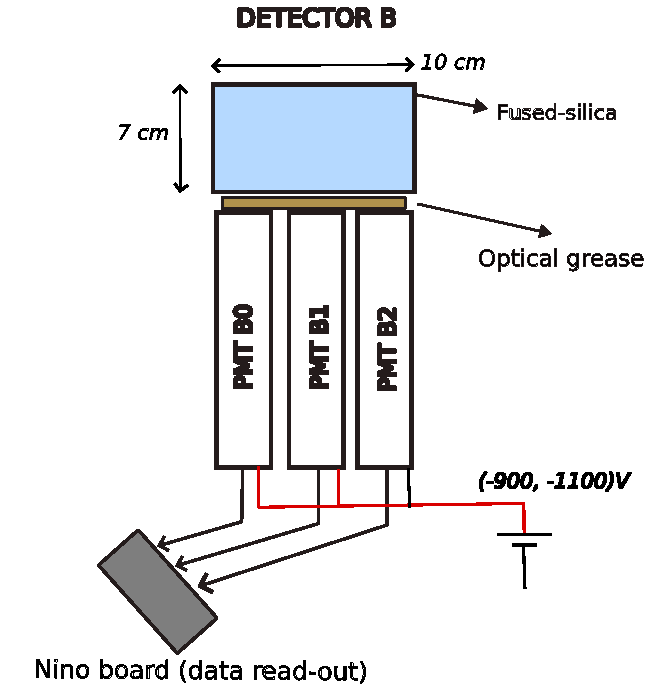
\includegraphics[width = 0.40\textwidth ]{ExperimentalSetup/Detectors/DetectorB.pdf}}
\subfloat[][\emph{Detector A scheme.}]{
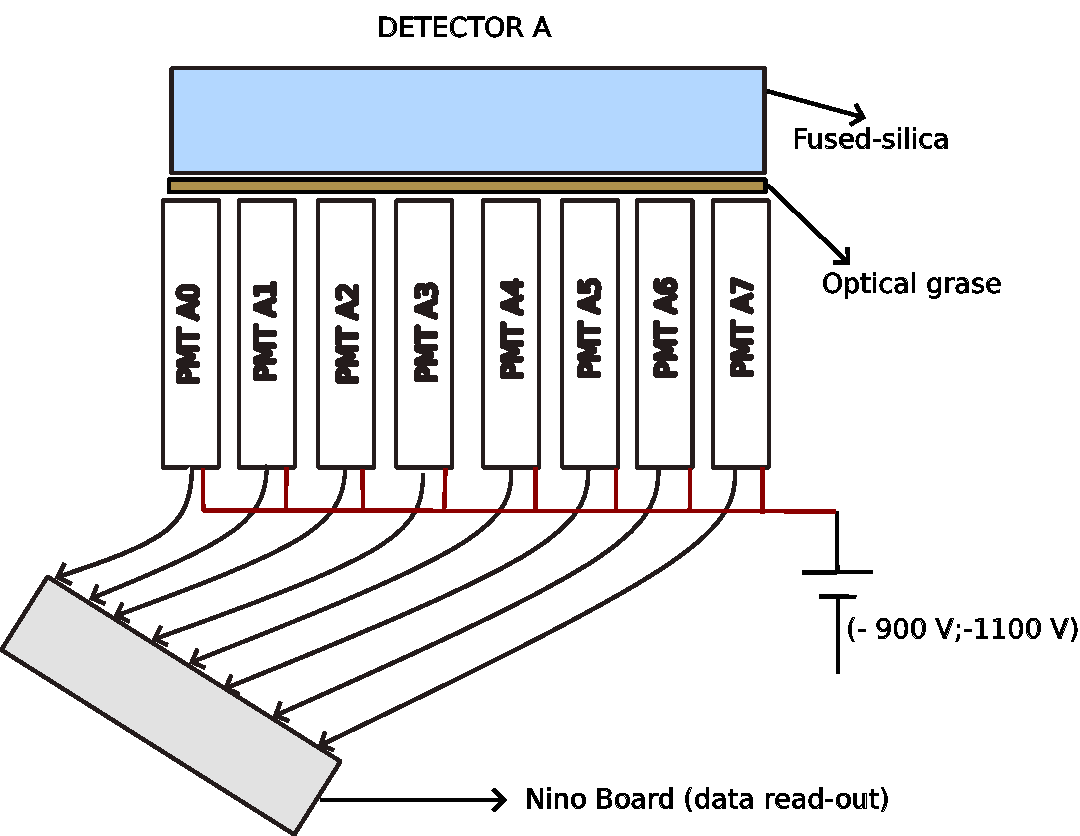
\includegraphics[width = 0.55\textwidth ]{ExperimentalSetup/Detectors/detectorA.pdf}}
\label{fig:NostriDetector}
\end{figure}

These two detectors are placed inside the spectrometers presented in \ref{fig:TwoDetectors}, between the top of the drift-chamber, which occupies the first third in height of the spectrometer, and just below the panel of scintillator. During the experiment, the drift chamber of the spectrometers is turn off, and also the PMTs coupled to the spectrometer scintillators are not powered.
As we mentioned above, the scattered electron are deflected in the vertical direction by the magnetic field of the spectrometer. It is important to mention the differences between the new and the old electronic setup. In the old electronic setup the output signal of the PMTs was integrated during the time interval of each sub-event, and therefore the single scattered electron could not be counted. The advantage of this method is that the electronics is simpler. However, this old method is affected by a baseline noise and it is not good for the future experiments with lead target, where the expected rates are lower than the rates on carbon.
With the new electronics, the single electrons are counted, and this will enable the future measurements with lead, improving the accuracy. 

\begin{figure}[hbtp]
\centering
\subfloat[][\emph{Detector B}]
	{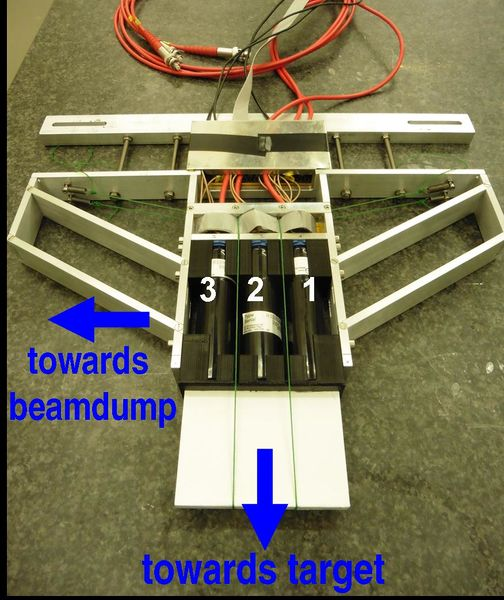
\includegraphics[width = 0.35\textwidth]{figures/504px-Blackfalcon.jpg}} \quad
\subfloat[][\emph{Detector A}]
	{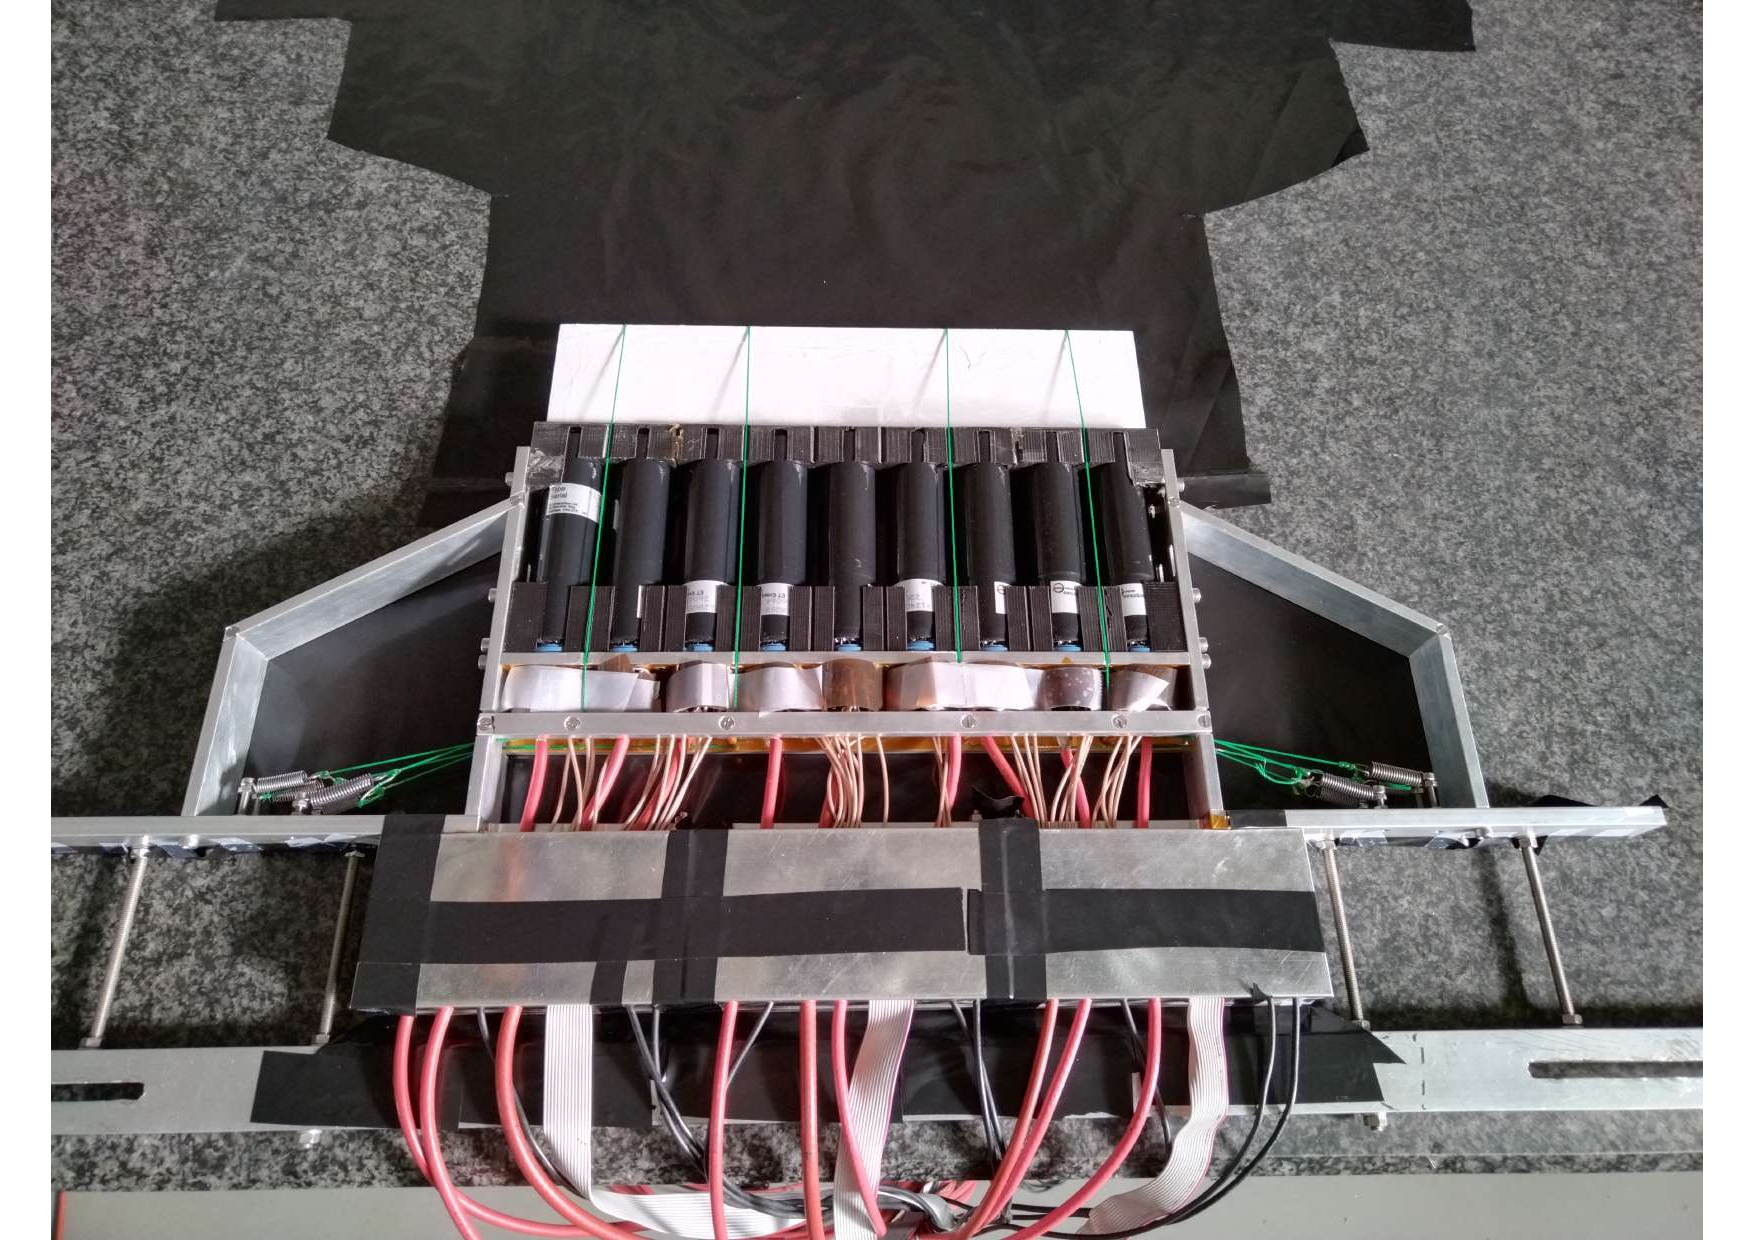
\includegraphics[width = 0.45\textwidth]{figures/IMG_20221110_122246.pdf}} \quad
	\label{fig:Detectors}
\caption{Picture of the two detector taken in the clean room. The white blocks are the fused silica that produces the Cherenkov light, the cylinders below are the PMTs.}
\end{figure}

Here we report the characteristic of the two detector that are relevant for the data analysis: 

\begin{itemize}
\item detector B size: $\SI{7}{\centi \meter} \times \SI{10}{\centi \meter} \times \SI{1}{\centi \meter}$
\item detector A size: $\SI{7}{\centi \meter} \times \SI{30}{\centi \meter} \times \SI{1}{\centi \meter}$
\item Number of dynodes of the PMT: 12
\item The Power voltage for the PMT in negative, in the range of ($\SI{-900}{\volt}$, $\SI{-1100}{\volt}$)
\item refraction index $n$ of the fused-silica is $1.45$.
\end{itemize}


\section{Beam Monitors}

In MAMI, several monitors are placed along the beam line to check the beam quality and measure parameters such as current intensity, energy and relative position of the beam. This section summarizes the operating principles of the monitors installed at MAMI. Some details will be given in the appendix, for a complete discussion please refer to the following paper \cite{M_Dehn}.
The monitors available at MAMI are constitutes by resonant cavities. With the resonant cavities it is possible to measure the various quantities, with the underlying physical principle that the passage of charged particles through these cavities can excitate some electromagnetic resonant modes\footnote{TM mode, where the magnetic field is completely transverse respect to particle momenta} which can be detected and analyzed by an analog circuit to measure the beam parameters.
Before going into the details, it is necessary to define some quantities that will be used later in the discussion. We define the Shunt-impedance $r_{s}$ as:

\begin{equation}
r_{s} = \frac{|V_{\|}|^{2}}{P}
\end{equation}

Where $P$ is the power absorbed by the cavity when a particle excites one of the resonant mode, and $V_{\|}$ is defined as the effective voltage experienced by a charged particle along a straight line, which can be computed as:

\begin{align*}
V_{\|} = \frac{1}{q}  \int_{s_{0}}^{s^{1}} \vec{E}_{s} \cdot  \,d \vec{s}
\end{align*}

The Shunt impedance is a measure of the interaction strength between a cavity and a charged particle, and can also be expressed using the $Q$ value of the cavity, the maximum energy stored $W$ and the frequency of resonance $f_{r}$:

\begin{align*}
r_{s} = \dfrac{|V_{\|}|^{2} Q}{2 \pi f_{r} W}
\end{align*}

When the beam travels through the cavity, the particles lose energy that excites the mode. The power $P_{HF}$ extracted from the beam is related to the beam current: 

\begin{equation}
P = i^{2} r_{s}
\end{equation}

An antenna is used to decouple part of the energy from the cavity and send it to a circuit which produces an analog output signal. Indicating with $\kappa$ the coupling constant of the antenna, the previous relation needs to be modified introducing a new factor $ \frac{\kappa}{(1 + \kappa)^2}$. In a cylindrical resonator, the type installed at MAMI, the resonance frequencies of the different oscillation modes are expressed by the formula: 

\begin{align*}
f_{m,n,p} = \frac{c}{2\pi \sqrt{\epsilon_{r} \mu_{r}}} \sqrt{\bigl(\frac{x_{m,n}}{R} \bigl)^{2} + \bigl(\frac{p \pi}{L} \bigl)^{2}}
\end{align*}

The constant in the formula are:

\begin{itemize}
\item $c$ is the light speed.
\item $\epsilon_{r}, \mu_{r}$ are the magnetic and dielectric constant of the material.
\item $x_{m,n}$ it the n-th zero of the m-th Bessel function.
\item $R$ and $L$ are the radius of the cylindrical cavity and his length.
\end{itemize}

This formula can be obtained solving the Maxwell equations with cylindrical boundary condition.
If the frequency of the beam bunch is equal to the resonant frequency $f_{m,n,p}$ of the cavity, a TM mode is excited. At MAMI high quality monitors are installed, with a $Q \simeq 10000$, that means that $\frac{\nu}{\delta \nu} \simeq 10000$. This means that the frequency of the beam buch must be very close to the frequency of the resonant cavity. At MAMI the frequency used for all the resonators is $\SI{2.449532}{\giga \hertz}$ or a multiple of it. The beam bunch frequency is the same, and it is controlled by the MAMI-master oscillation signal, that is the reference signal for all the MAMI monitors.

\begin{figure}[hbtp]
\centering
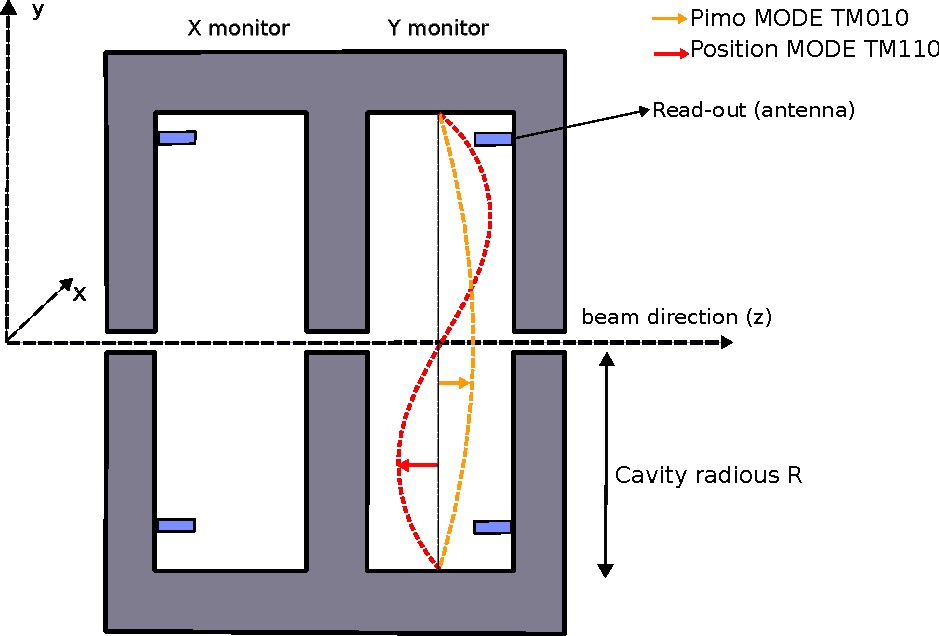
\includegraphics[width = 0.6 \textwidth]{ExperimentalSetup/Monitors.pdf}
\caption{Scheme of the Cylindrical cavities installed at MAMI. In red we have the $TM_{110}$ mode, used to measure the position of the beam, in yellow the $TM_{010}$ mode, to measure the intensity of the beam.}
\end{figure}

Depending on the $TM$ mode excited, we have a different signal in the cavity, so a different signal collected by the antenna. The relevant quantity that is detected is the power $P_{HF}$ absorbed by the antenna. For the $TM_{010}$ mode, the power is 

\begin{equation}
P_{HF} = i^{2} r_{010} \frac{\kappa}{(1 + \kappa)^{2}}
\end{equation}

The power absorbed by the antenna is directly dependent on the beam current. Because the values are typically in the range of $\SI{}{\pico \watt}$ to $\SI{}{\milli \watt }$, the signal is processed in close proximity of the installed monitors. In the signal processing, the input signal of the antenna in coupled to the master-oscillation signal, so the output signal is given by the formula:

\begin{equation}
U = \sqrt{P_{HF}} \cos(\phi - \phi_{LO})
\end{equation}

where the phase $\phi$ is the phase of the resonant mode or the phase of the beam bunch, while the phase $\phi_{LO}$ is the phase respect to the master-oscillation signal, and can be adjusted by a phase shifter in the circuit. The output voltage signal can be read out with the oscilloscope or digitalized and saved with other devices. To measure the beam intensity is important to minimize $\phi - \phi_{LO}$ (see figure \ref{fig:PIMO}), to maximize the signal amplitude.

\begin{figure}[hbtp]
\centering
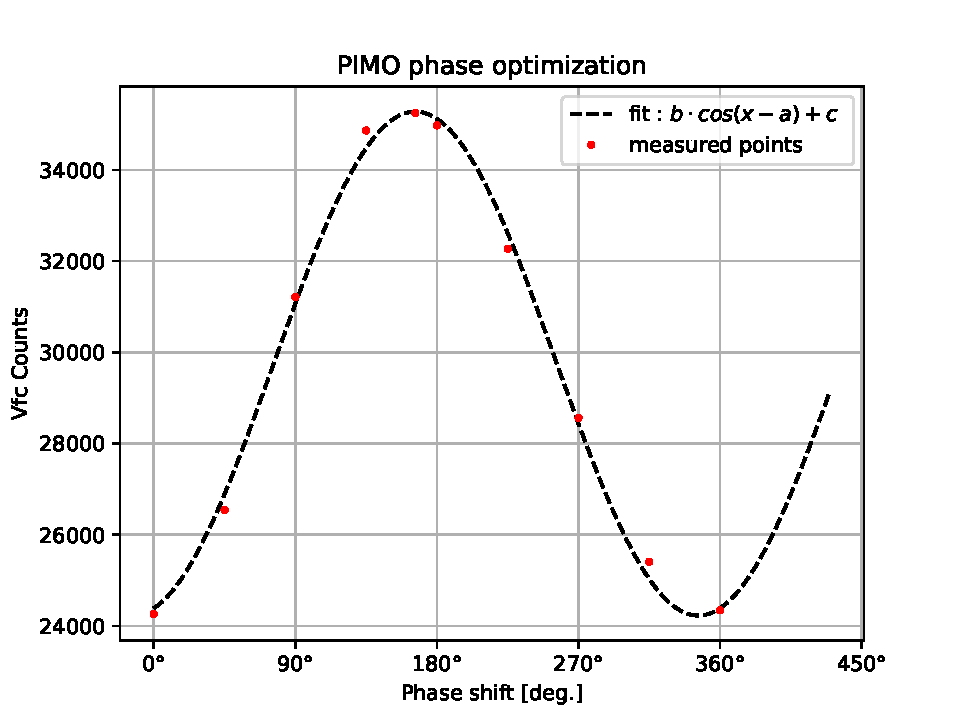
\includegraphics[width = 0.5\textwidth]{ExperimentalSetup/PIMOphase.pdf}
\caption{Plot of the phase $\phi$ versus the output signal. The phase optimization was done selecting the working point in correspondence of the peak.}
\label{fig:PIMO}
\end{figure}

The measurement of the $x,y$ position follows in principle the same procedure. In this case the $TM_{110}$ is acquired. The reason is clear, because it is possible to calculate that for this mode the $r_{shunt}$ is proportional to the beam position on the $x,y$ plane. So The power absorbed by the antenna can be written:

\begin{equation}
P_{HF} = i^{2} r_{110} \frac{\kappa}{(1 + \kappa)^{2}} K x^{2}
\end{equation} 
 
The output signal, that is read by our setup, is proportional to the square root of the absorbed power:

\begin{equation}
\sqrt{P_{HF}} = constant \cdot U \, \cdot \, i   \cdot x
\end{equation} 

The beam parameter are then given inverting the above formula 

\begin{equation} \label{eq:SignalToVfc}
x \simeq \frac{\sqrt{P_{HF}}}{i}
\end{equation}

Where the exact conversion coefficients are not known, and are determined during the calibration phase, at the beginning of the beam time.
To measure the beam energy, a different approach is used. The energy monitor (ENMO) consist of 2 cavities in the RTM3. One is located in the last recirculation pipe, the other one on the part of the beam line, where the acceleration takes place. The two monitors are synchronized to the master oscillation and measure the phase of the bunches of electrons. During their travel from the first cavity to the second cavity, the beam passes through the magnet and does one half turn. If the energy is slightly higher, the radius of the turn will be slightly larger. This means that there is an extra time between the two bunches, that can be measured as a small phase shift in the $\SI{570}{\mega \electronvolt}$ recirculation. From this it is possible to obtain a value for the difference of the actual energy from the nominal energy.

\subsection{Beam stabilization}

The beam stabilization is an essential component of the experiment. The values of $A_{n}$ that we want to measure are in the order of ten $ppm$, so it is important to reduce other contributions that can be related to variations in the beam parameters. 

\section{Electronics}
\commento{Short introduction about the old electronics setup and why a new versions is needed, then describe all the electronics used for our experiment:
\begin{itemize}
\item Nino board for collecting the data from the PMTs
\item VFCs for collecting the data from X21,X25,Y21,Y25,ENMO,I21,I13
\item master board for collecting the monitors data/controlling the source/wobbler magnets.
\item small boxes for switching from new electronic read-out to the old electronics read-out (spectrometers DAQ)
\end{itemize}}


\subsection{Voltage to Frequency Converter}

Some beam parameters are needed in order to take into account possible effects in the measurement of the transverse asymmetry. The relevant data are the position in the $(x,y)$ plane, the incident angles on the target, the current and energy of the beam. All this values are collected using the already existing monitors.
To collect the data from the monitors, single and multichannel, synchronous voltage-to-frequency converters (AD7742) are used. This devices contain an analog modulator that is able to convert the input voltage into an output pulse train, whose frequency is proportional to the input voltage. 

\begin{wrapfloat}{figure}{I}{0pt}
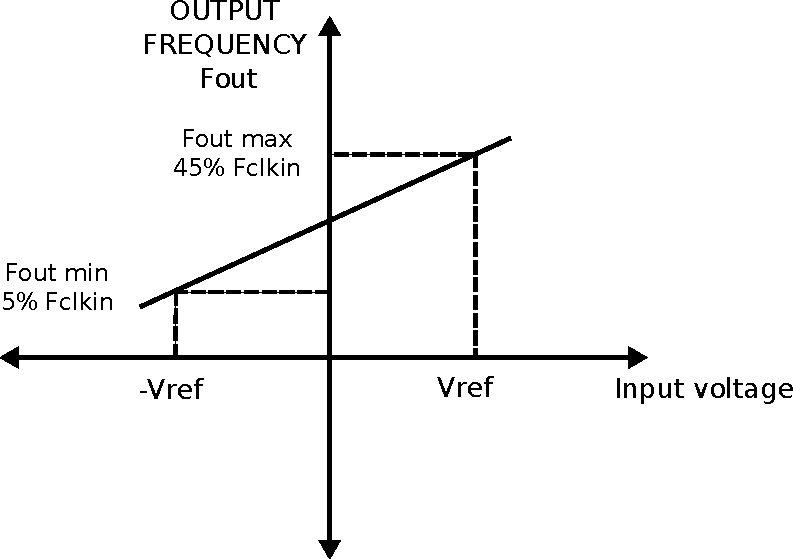
\includegraphics[width=0.5\textwidth]{ExperimentalSetup/Vfc.pdf}
\caption{Frequency versus Voltage}
\vspace{10pt}
\end{wrapfloat}

The VFCs are powered with an external voltage of $\SI{5}{\volt}$. They measure an input voltage in the range of ($-V_{ref}$, $V_{ref}$). An external clock signal, with a frequency $F_{CLKIN} = \SI{5.88}{\mega \hertz}$ is created externally and synchronous to the gate-length.
The analog input signal is sampled with by a switched capacitor, with a rate that is equal to $F_{CLKIN}$.
The comparator produces a number pulses; the frequency of the output signal is proportional to the input voltage, with $-V_{ref}$ equal to $0.5 \% \cdot f_{CLKIN}$ and $+V_{ref}$ equal to $0.45 \% \cdot f_{CLKIN}$ \cite{VfcDatasheet}, where the first correspond to $\SI{0.0}{ \volt}$ in input and the second to $V_{ref}$. The relation between the output frequency and the input voltage is the following:

\begin{equation}
V_{in} = V_{ref} (2 \frac{f_{out} - 5\% F_{CLKIN}}{40 \% \cdot F_{CLKIN}} -1)
\end{equation}

The data are acquired counting the number of pulses that come from the comparator, so we can substitute to $f$ the number of pulses (the two quantities are proportional), and we end with:

\begin{equation} \label{eq:Vfc}
V_{in} =  V_{ref}[2 \cdot \dfrac{N_{pulses} - 5 \% N_{CLKN}}{40 \% N_{CLKN}} - 1]
\end{equation}

\subsection{Nino Board} \label{NINO}

The NINO board is our data acquisition system for the PMT counts. It is made by $32$ analog input channels and it is powered with $\pm \SI{5}{\volt}$. Each channel has an attenuator, and the signal passes through that before going to the comparator, which compares the signal to the threshold. The output signal is a Low-voltage differential signal (LVDS). Each comparator can handle eight channels and for each of them it is possible to define a global threshold. 
The threshold of the NINO board can be controlled with two values, that are named threshold \textit{Thr} and attenuation \textit{Att}. A \textit{Thr} value is shared by 4 adjacent channels, while each channel has is own value of \textit{Att}. In this way it is possible to define a different vale of the threshold for each individual channel. The \textit{Att} value decrease the global threshold selected with \textit{Thr}. These two parameters are set in the DAQ program, using 12 bit DACs, corresponding to interval of $(0 ; 4095)$.
The NINO board is designed in such a way that collects the Input charge of the signal, operating with a $\SI{30}{\pico \farad}$ capacitor. The output signal amplitude is proportional to the input charge, and it is sent to the discriminator. Our interest is only to count the number of scattered electron, so we do not intend to measure the input charge, but only if a signal is produced or not.

\begin{figure}[hbtp]
\centering
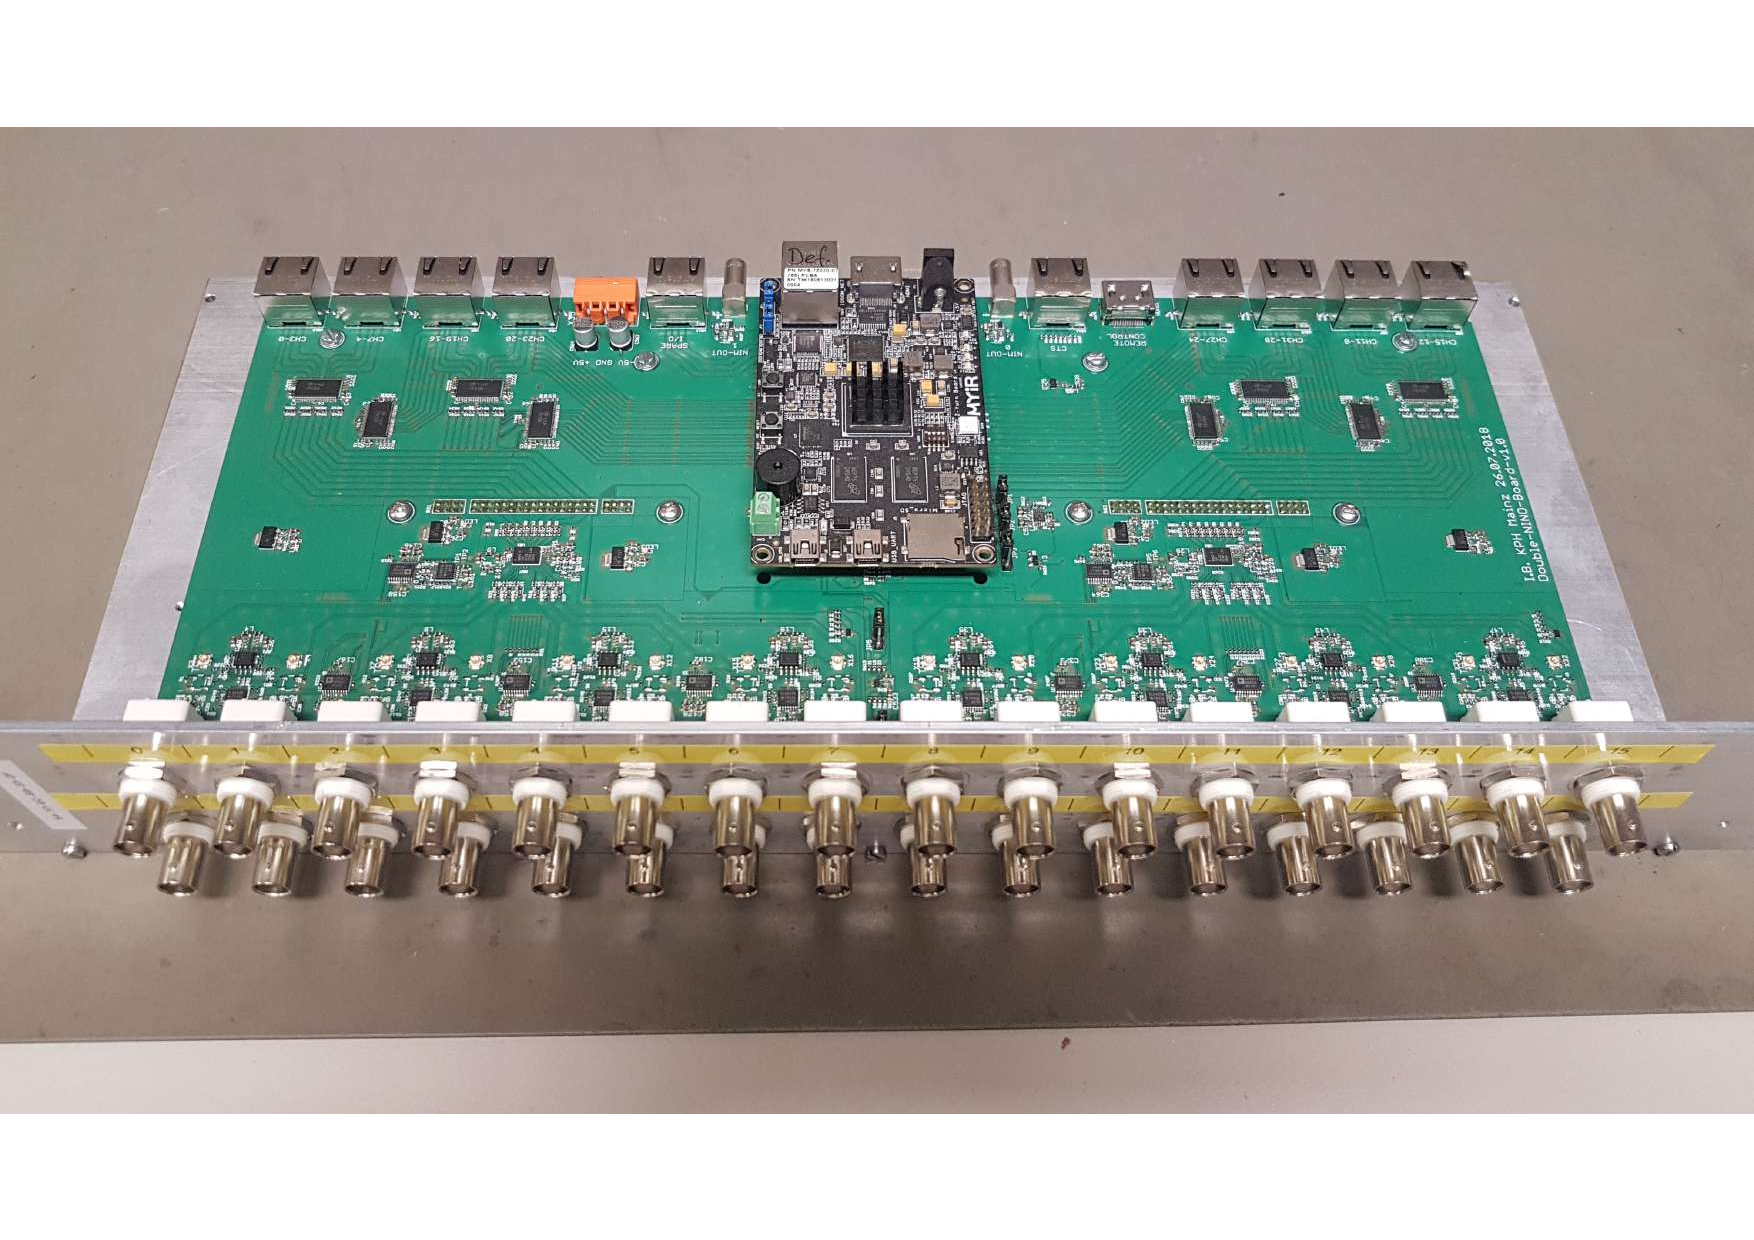
\includegraphics[width = 0.75\textwidth]{ExperimentalSetup/NINO.pdf}
\caption{Nino Board}
\label{fig:NinoBoard}
\end{figure}

Two Nino board are used in the experiment, one for detector A and one for detector B. For the experiment discussed in this thesis, we will use only 8 channel for detector A and 3 channel for detector B, since this is the number of the input signals coming from the two detectors. For the future experiments more channel will be used, splitting the analog input signal in 4 different signal, sending it to 4 different input channel of the board. This is useful because changing individually the attenuation value, we can define 4 different thresholds for the same signal coming from a single PMT, and compare different values of threshold, for example to study how the noise affects the measurement, finding the best compromise between signal to noise ratio.
The way we selected the threshold is explained in chapter.

\subsection{Master Board}

\begin{figure}[hbtp]

\centering
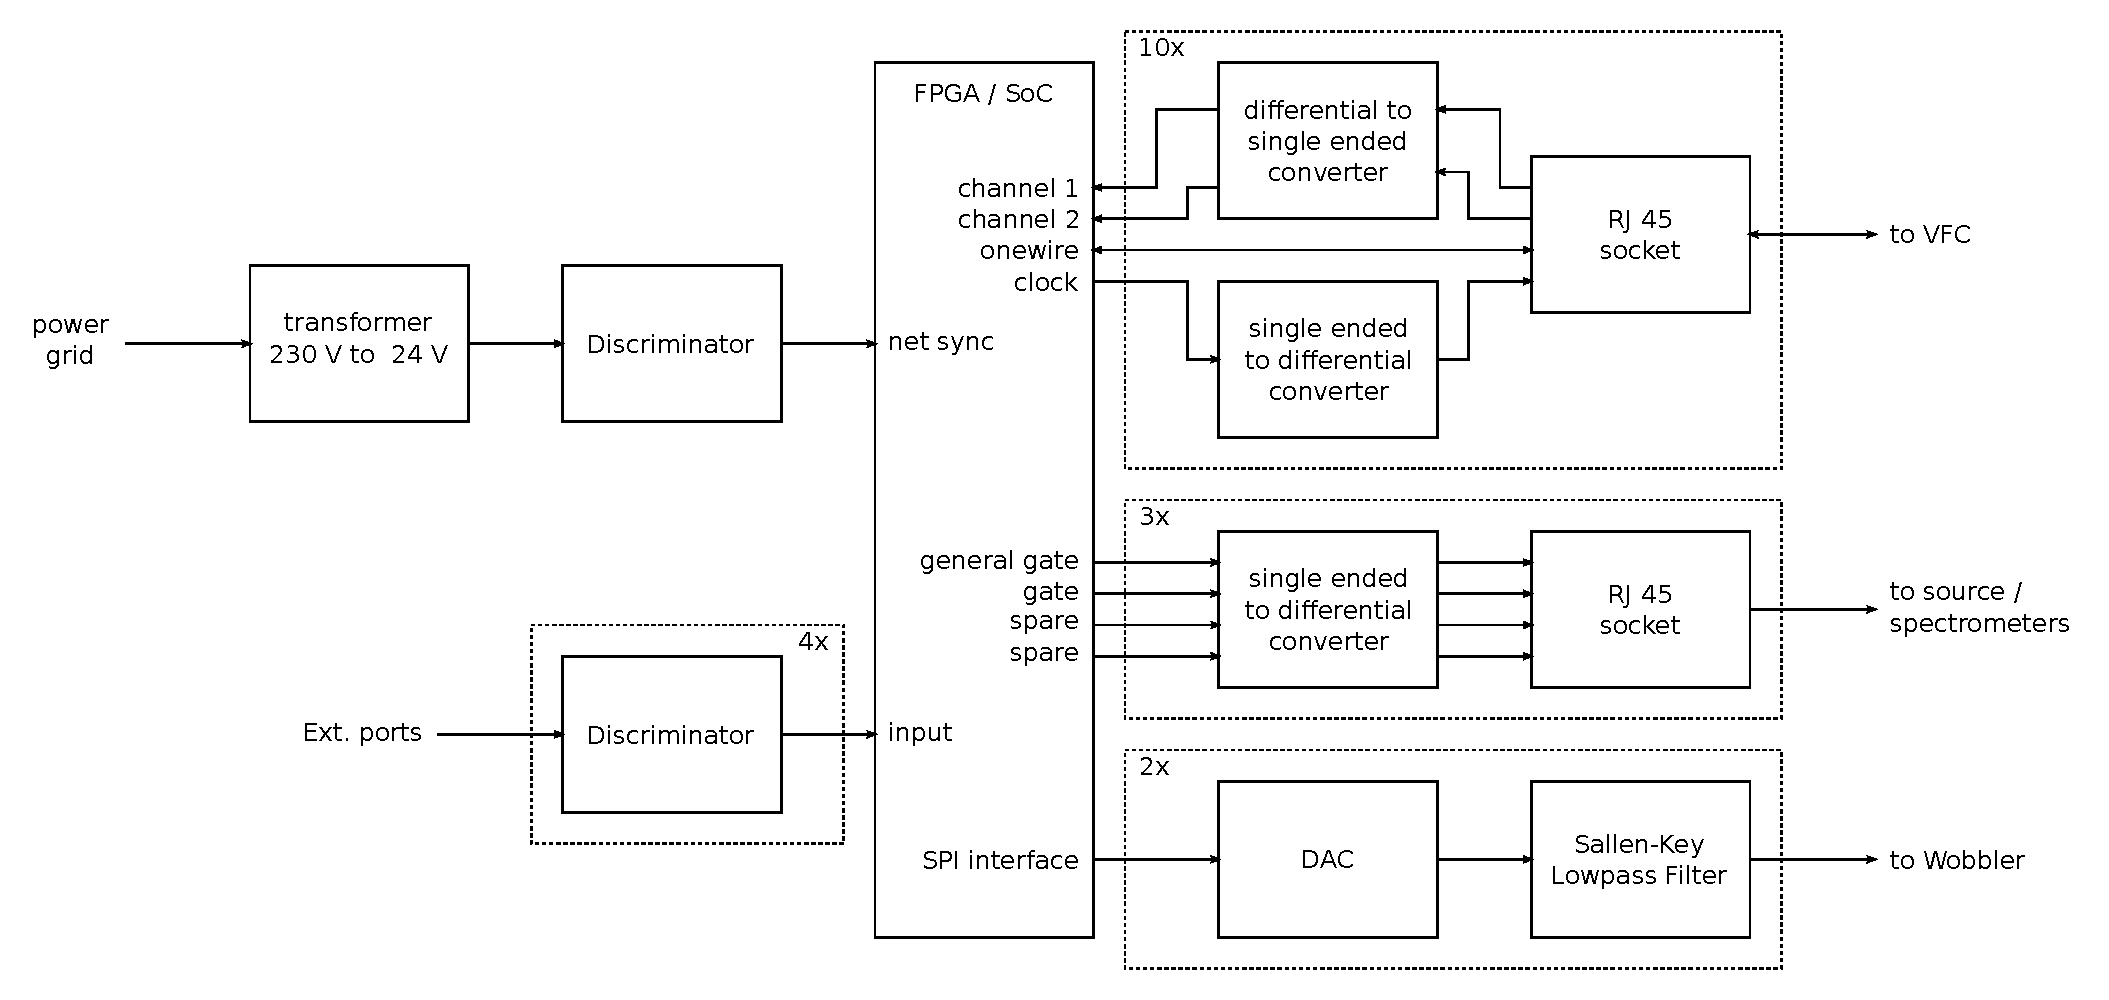
\includegraphics[width = \textwidth]{ExperimentalSetup/masterboard.pdf}
\caption{Scheme of the master-board, the device that coordinates all the electronics for the experiments, and send the data to the computer in the control room.}
\end{figure}

